\documentclass{beamer}
\usepackage[latin1]{inputenc}
\usepackage{times}
\usepackage{tikz}
\usetheme{Luebeck}
%\usecolortheme{albatross}
\usepackage{amsmath,amsfonts,amsthm,amssymb}
\usepackage{setspace}
\usepackage{Tabbing}
\usepackage{fancyhdr}
\usepackage{lastpage}
\usepackage{extramarks}
\usepackage{chngpage}
\usepackage{soul,color}
\usepackage{graphicx,float,wrapfig}
\usepackage{xcolor}
\usepackage{listings}
\usepackage{float}
%\usepackage{subfloat}
\usepackage{subfig}
\usepackage{caption}
\usepackage{enumitem}
\usepackage{algpseudocode}

\definecolor{darkorange}{RGB}{240, 120, 0}
\definecolor{darkgreen}{RGB}{0, 128, 0}

\setbeamercolor{background canvas}{bg=white}
\setbeamercolor{frametitle}{fg=white, bg=darkorange}
\setbeamercolor{normal text}{bg=black,fg=black}
\setbeamercolor{structure}{bg=black, fg=darkorange}

\title{Lecture 7: Image Sources, Convolution, Scene Graphs}
\date{2/4/2016}
\institute{Chris Tralie, Duke University}
\author{COMPSCI/MATH 290-04}
\begin{document}

\frame{\titlepage}

\begin{frame}{Announcements}

\begin{itemize}[label=$\blacktriangleright$]
    \item Mini Assignment 2 Due Next Monday 11:55 PM
    \item Group Assignment 1 will be released before Monday
    \item Find partners!
\end{itemize}

\end{frame}

\begin{frame}{Table of Contents}

\begin{itemize}[label=$\blacktriangleright$]
	\item 3D Rotations Continued
\end{itemize}
\begin{itemize}[label=$\vartriangleright$]
    \item Image Sources
	\item Convolution
	\item Scene Graphs
\end{itemize}

\end{frame}

\begin{frame}{3D Rotations: Coordinate Frame Interpretation}

\begin{figure}[t]
    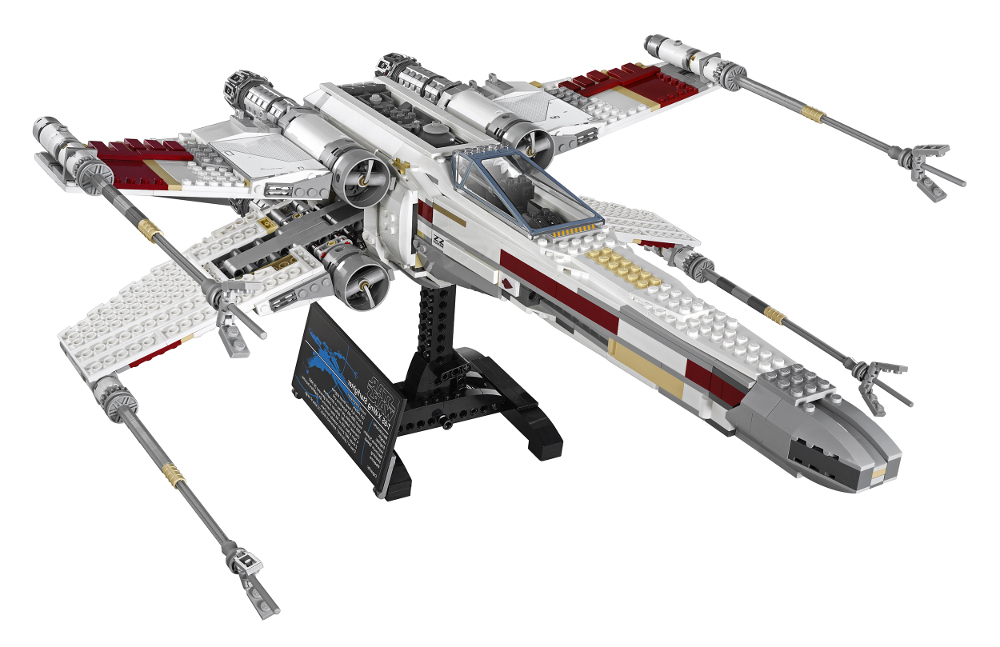
\includegraphics[width=0.6\textwidth]{XWing.jpg}
\end{figure}

\end{frame}


\begin{frame}{3D Rotations: Euler Angles Visualization}

\end{frame}

\begin{frame}{Table of Contents}


\begin{itemize}[label=$\vartriangleright$]
	\item 3D Rotations Continued
\end{itemize}
\begin{itemize}[label=$\blacktriangleright$]
    \item Image Sources
\end{itemize}
\begin{itemize}[label=$\vartriangleright$]
	\item Convolution
	\item Scene Graphs
\end{itemize}

\end{frame}


\begin{frame}{Ray Casting for Specular Reflections}

\begin{figure}[t]
	\centering
    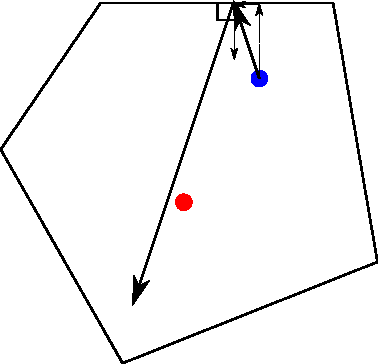
\includegraphics[width=0.46\textwidth]{ImageSources1.pdf}
\end{figure}

\begin{itemize}[label=$\vartriangleright$]
\item Project onto normal, flip normal component, preserve parallel component
\end{itemize}

\end{frame}


\begin{frame}{Ray Casting for Specular Reflections}

\begin{figure}[t]
	\centering
    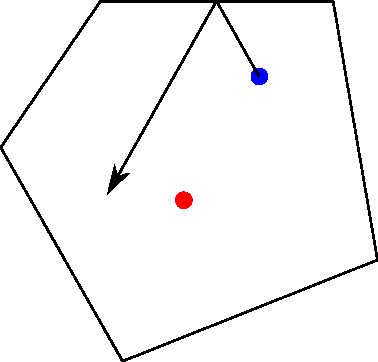
\includegraphics[width=0.46\textwidth]{ImageSources2.pdf}
\end{figure}

\end{frame}

\begin{frame}{Ray Casting for Specular Reflections}

\begin{figure}[t]
	\centering
    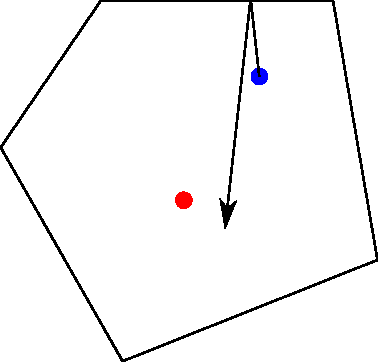
\includegraphics[width=0.46\textwidth]{ImageSources3.pdf}
\end{figure}

\end{frame}

\begin{frame}{Ray Casting for Specular Reflections}

\begin{figure}[t]
	\centering
    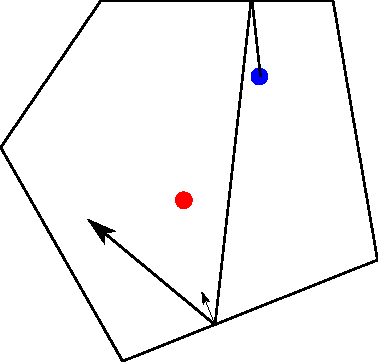
\includegraphics[width=0.46\textwidth]{ImageSourcesMulti1.pdf}
\end{figure}

\end{frame}

\begin{frame}{Ray Casting for Specular Reflections}

\begin{figure}[t]
	\centering
    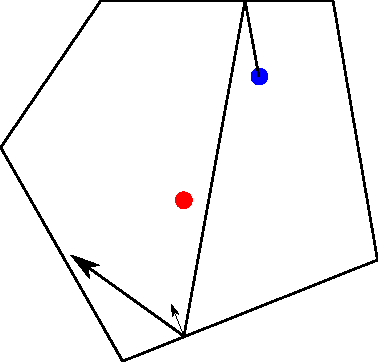
\includegraphics[width=0.46\textwidth]{ImageSourcesMulti2.pdf}
\end{figure}

\end{frame}

\begin{frame}{Ray Casting for Specular Reflections}

\begin{figure}[t]
	\centering
    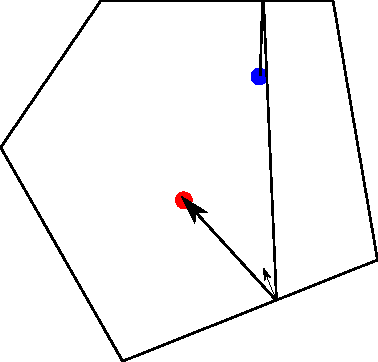
\includegraphics[width=0.46\textwidth]{ImageSourcesMulti3.pdf}
\end{figure}

\end{frame}

\begin{frame}{Ray Casting for Specular Reflections}

\begin{figure}[t]
	\centering
    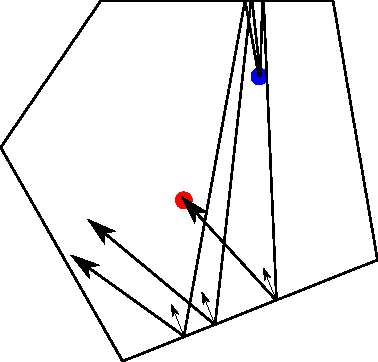
\includegraphics[width=0.46\textwidth]{ImageSourcesMulti.pdf}
\end{figure}

\begin{itemize}[label=$\vartriangleright$]
    \item Dilution of precision
    \item Need fine angle resolution to capture!
\end{itemize}

\end{frame}

\begin{frame}{Image Sources}

\begin{figure}[t]
	\centering
    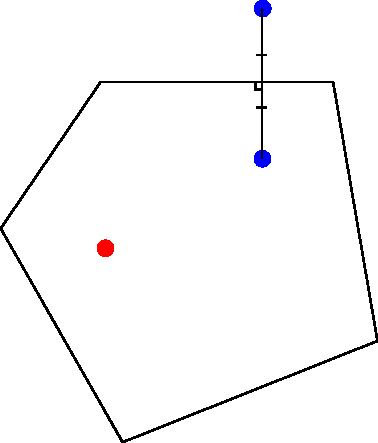
\includegraphics[width=0.6\textwidth]{ImageSourcesDrawn0.pdf}
\end{figure}

\end{frame}

\begin{frame}{Image Sources}

\begin{figure}[t]
	\centering
    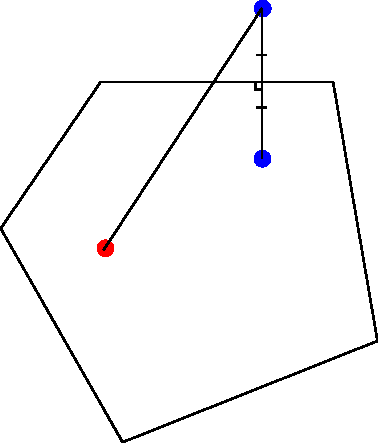
\includegraphics[width=0.6\textwidth]{ImageSourcesDrawn1.pdf}
\end{figure}

\end{frame}

\begin{frame}{Image Sources}

\begin{figure}[t]
	\centering
    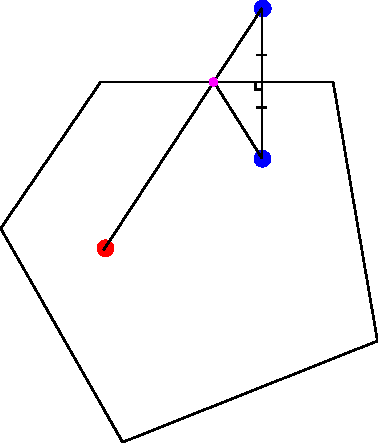
\includegraphics[width=0.6\textwidth]{ImageSourcesDrawn2.pdf}
\end{figure}

\end{frame}

\begin{frame}{Image Sources: Proof}

\begin{figure}[t]
	\centering
    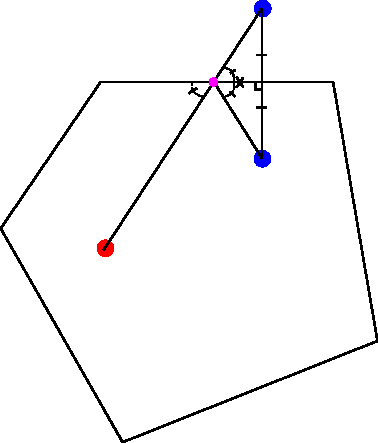
\includegraphics[width=0.6\textwidth]{ImageSourcesDrawn3Proof.pdf}
\end{figure}

\end{frame}

\begin{frame}{Image Sources: More Examples}

\begin{figure}[t]
	\centering
    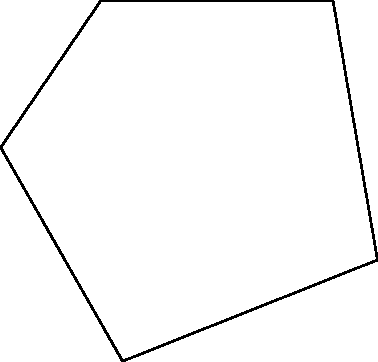
\includegraphics[width=0.6\textwidth]{ImageSourcesMoreExamples.pdf}
\end{figure}

\end{frame}


\begin{frame}{Image Sources: Second Order}

\begin{figure}[t]
	\centering
    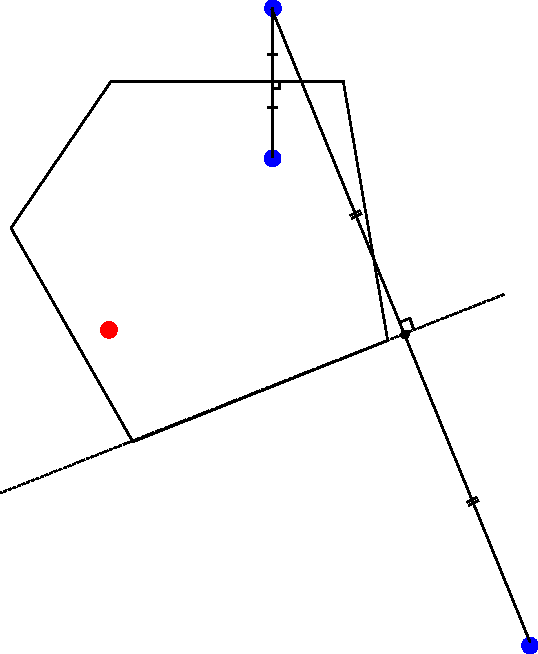
\includegraphics[width=0.5\textwidth]{ImageSourcesMultiDrawn0.pdf}
\end{figure}

\end{frame}

\begin{frame}{Image Sources: Second Order}

\begin{figure}[t]
	\centering
    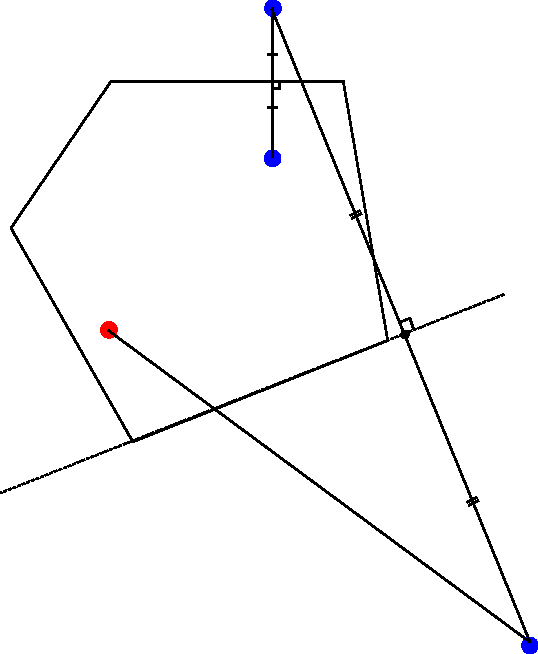
\includegraphics[width=0.5\textwidth]{ImageSourcesMultiDrawn1.pdf}
\end{figure}

\end{frame}

\begin{frame}{Image Sources: Second Order}

\begin{figure}[t]
	\centering
    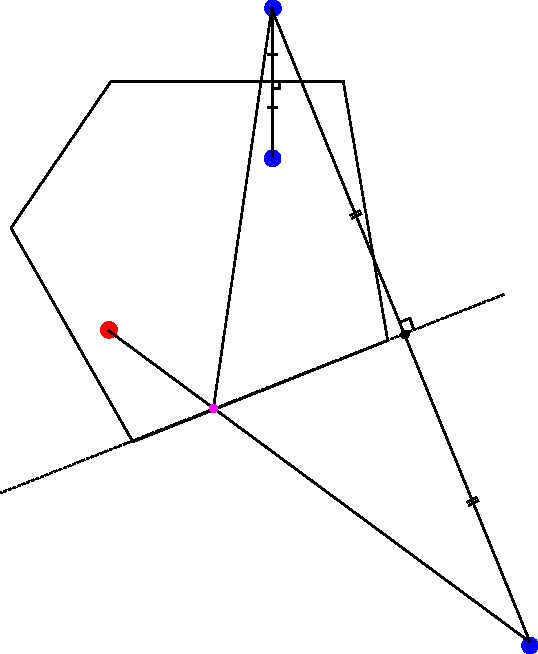
\includegraphics[width=0.5\textwidth]{ImageSourcesMultiDrawn2.pdf}
\end{figure}

\end{frame}

\begin{frame}{Image Sources: Second Order}

\begin{figure}[t]
	\centering
    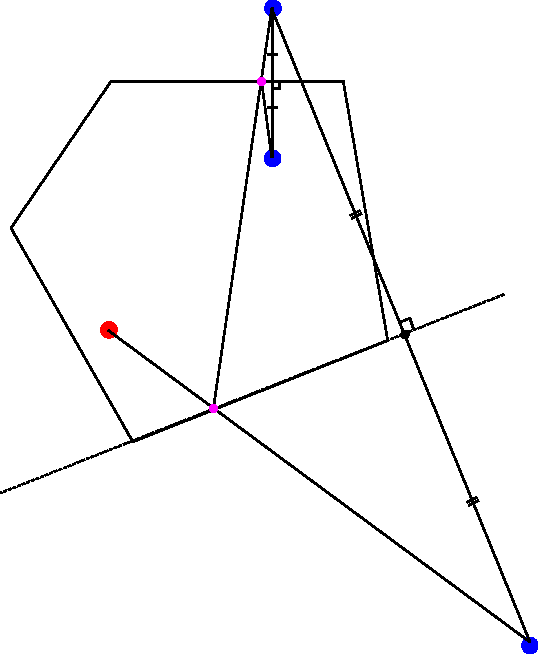
\includegraphics[width=0.5\textwidth]{ImageSourcesMultiDrawn3.pdf}
\end{figure}

\end{frame}

\begin{frame}{Image Sources: Third Order (!)}

\begin{figure}[t]
	\centering
    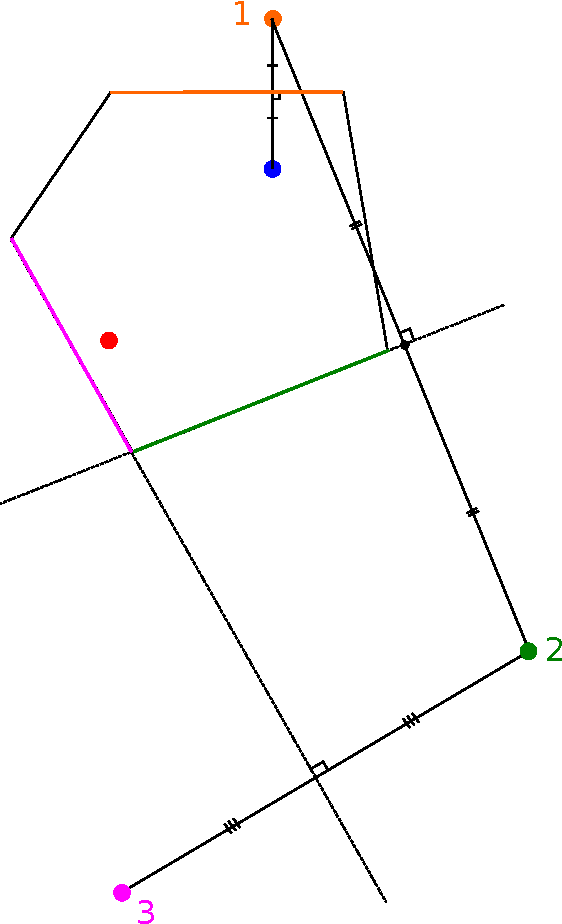
\includegraphics[width=0.43\textwidth]{ImageSources2MultiDrawn0.pdf}
\end{figure}

\end{frame}

\begin{frame}{Image Sources: Third Order}

\begin{figure}[t]
	\centering
    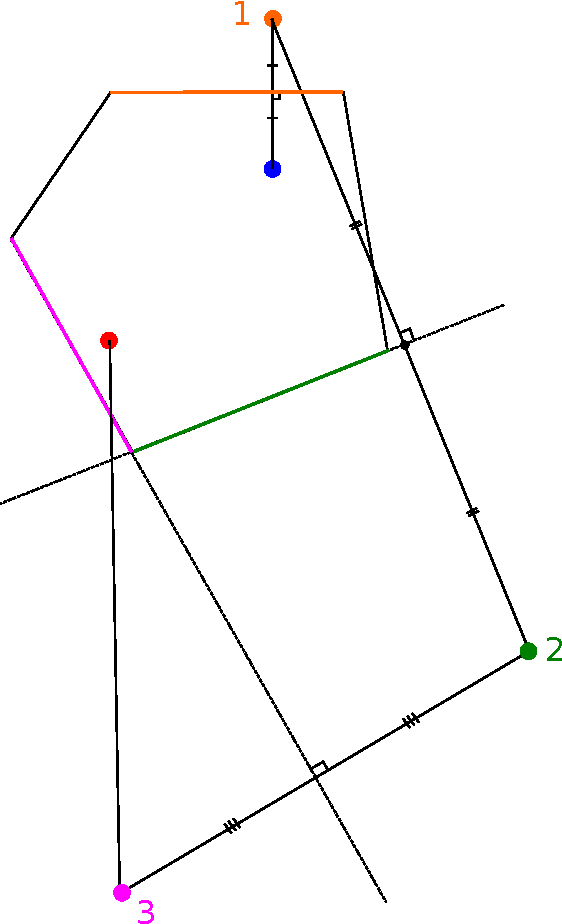
\includegraphics[width=0.43\textwidth]{ImageSources2MultiDrawn1.pdf}
\end{figure}

\end{frame}


\begin{frame}{Image Sources: Third Order}

\begin{figure}[t]
	\centering
    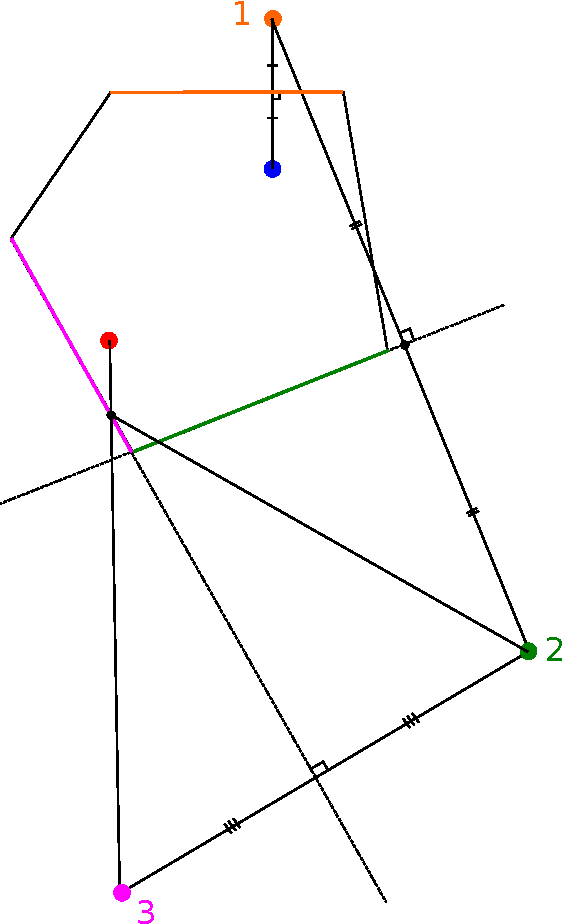
\includegraphics[width=0.43\textwidth]{ImageSources2MultiDrawn2.pdf}
\end{figure}

\end{frame}

\begin{frame}{Image Sources: Third Order}

\begin{figure}[t]
	\centering
    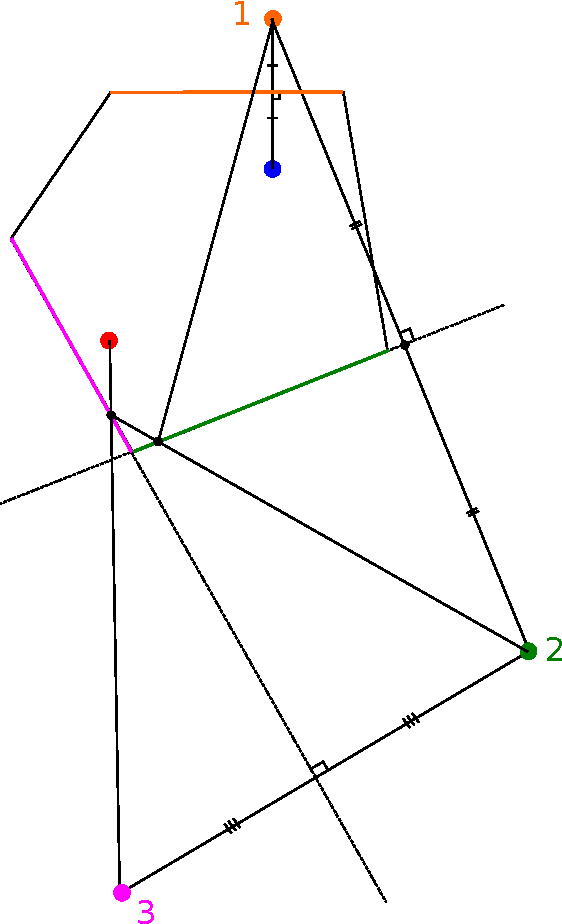
\includegraphics[width=0.43\textwidth]{ImageSources2MultiDrawn3.pdf}
\end{figure}

\end{frame}

\begin{frame}{Image Sources: Third Order}

\begin{figure}[t]
	\centering
    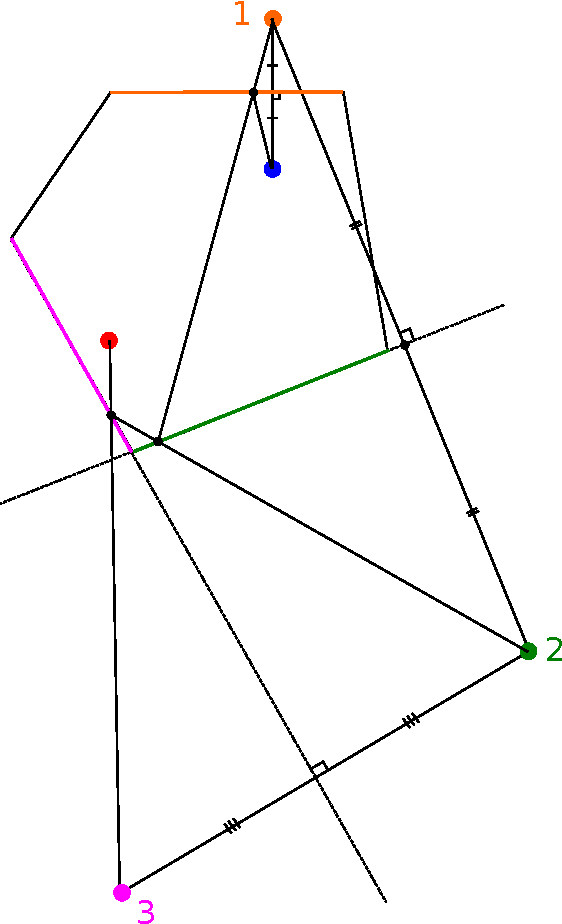
\includegraphics[width=0.43\textwidth]{ImageSources2MultiDrawn4.pdf}
\end{figure}

\end{frame}

\begin{frame}{Image Sources: Third Order}

\begin{figure}[t]
	\centering
    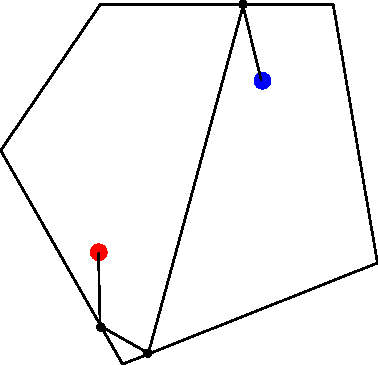
\includegraphics[width=0.7\textwidth]{ImageSources2MultiDrawn5.pdf}
\end{figure}

\end{frame}

\begin{frame}{Image Sources: Occlusions}

\begin{figure}[t]
	\centering
    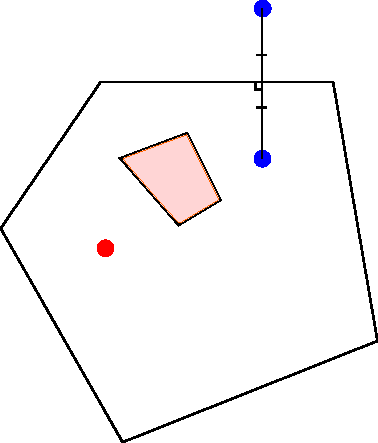
\includegraphics[width=0.55\textwidth]{ImageSourcesOcclusion.pdf}
\end{figure}

\end{frame}

\begin{frame}{Image Sources: Occlusions}

Ray needs to hit target before anything else

\begin{figure}[t]
	\centering
    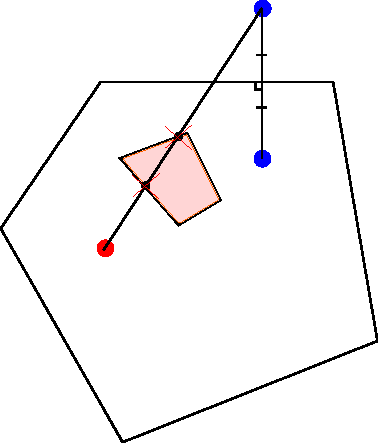
\includegraphics[width=0.55\textwidth]{ImageSourcesOcclusions2.pdf}
\end{figure}



\end{frame}


\begin{frame}{Image Sources: Point Containment}

\begin{figure}[t]
	\centering
    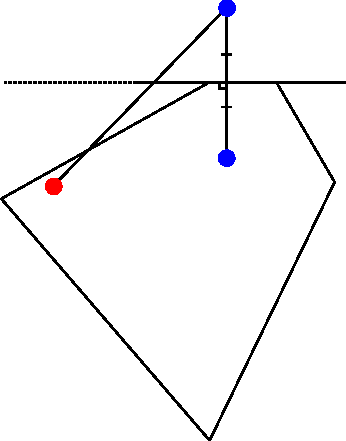
\includegraphics[width=0.5\textwidth]{ImageSourcesInsideSegment.pdf}
\end{figure}

\end{frame}

\begin{frame}{Image Sources: Point Containment}

Intersection with line (plane in 3D) must be in interior of polygon

\begin{figure}[t]
	\centering
    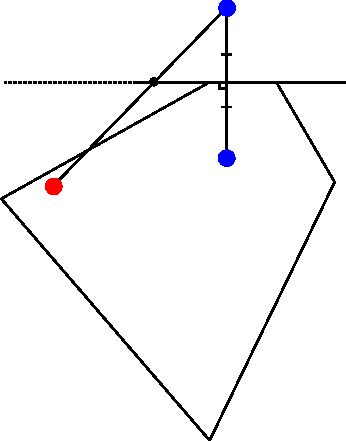
\includegraphics[width=0.5\textwidth]{ImageSourcesInsideSegment1.pdf}
\end{figure}

\end{frame}

\begin{frame}{Table of Contents}
\begin{itemize}[label=$\vartriangleright$]
	\item 3D Rotations Continued
    \item Image Sources
\end{itemize}
\begin{itemize}[label=$\blacktriangleright$]
	\item Convolution
\end{itemize}
\begin{itemize}[label=$\vartriangleright$]
	\item Scene Graphs
\end{itemize}

\end{frame}


\begin{frame}{Impulse Response}

\begin{itemize}[label=$\vartriangleright$]
\item Convert lengths of all paths into times, amplitude records decay
\end{itemize}

\begin{figure}[t]
	\centering
    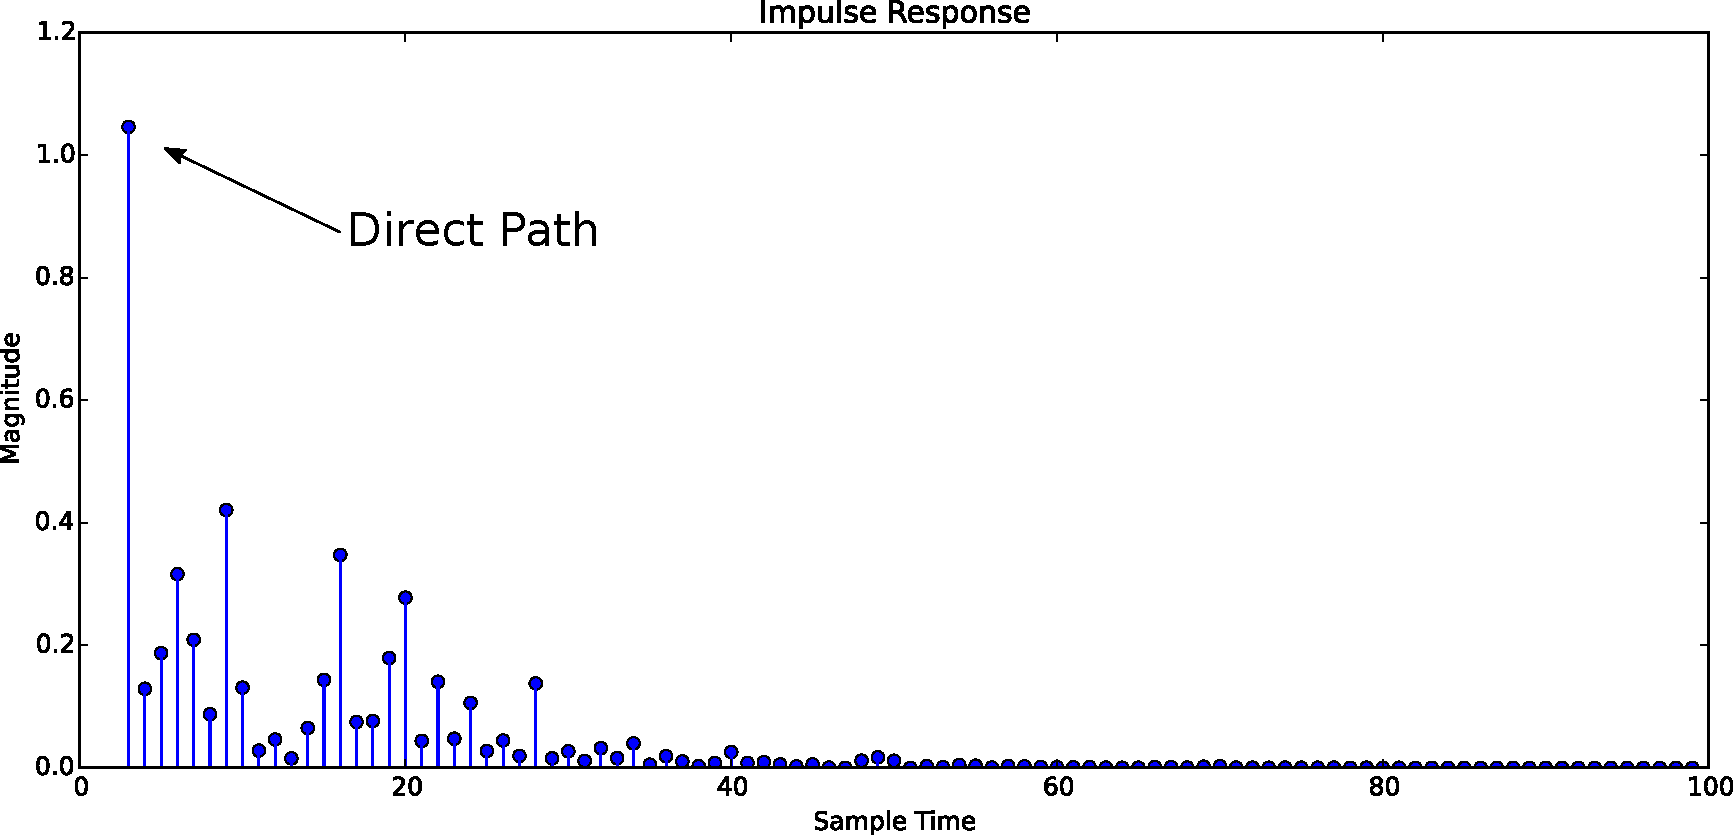
\includegraphics[width=\textwidth]{ImpulseResponse.pdf}
\end{figure}

\uncover<2->{
\begin{itemize}[label=$\vartriangleright$]
\item What causes decay?
\end{itemize}
}

\end{frame}


\begin{frame}{Convolution}

\begin{itemize}[label=$\vartriangleright$]
\item Convolution: What do sounds sound like in this environment?
\end{itemize}

\begin{figure}[t]
	\centering
    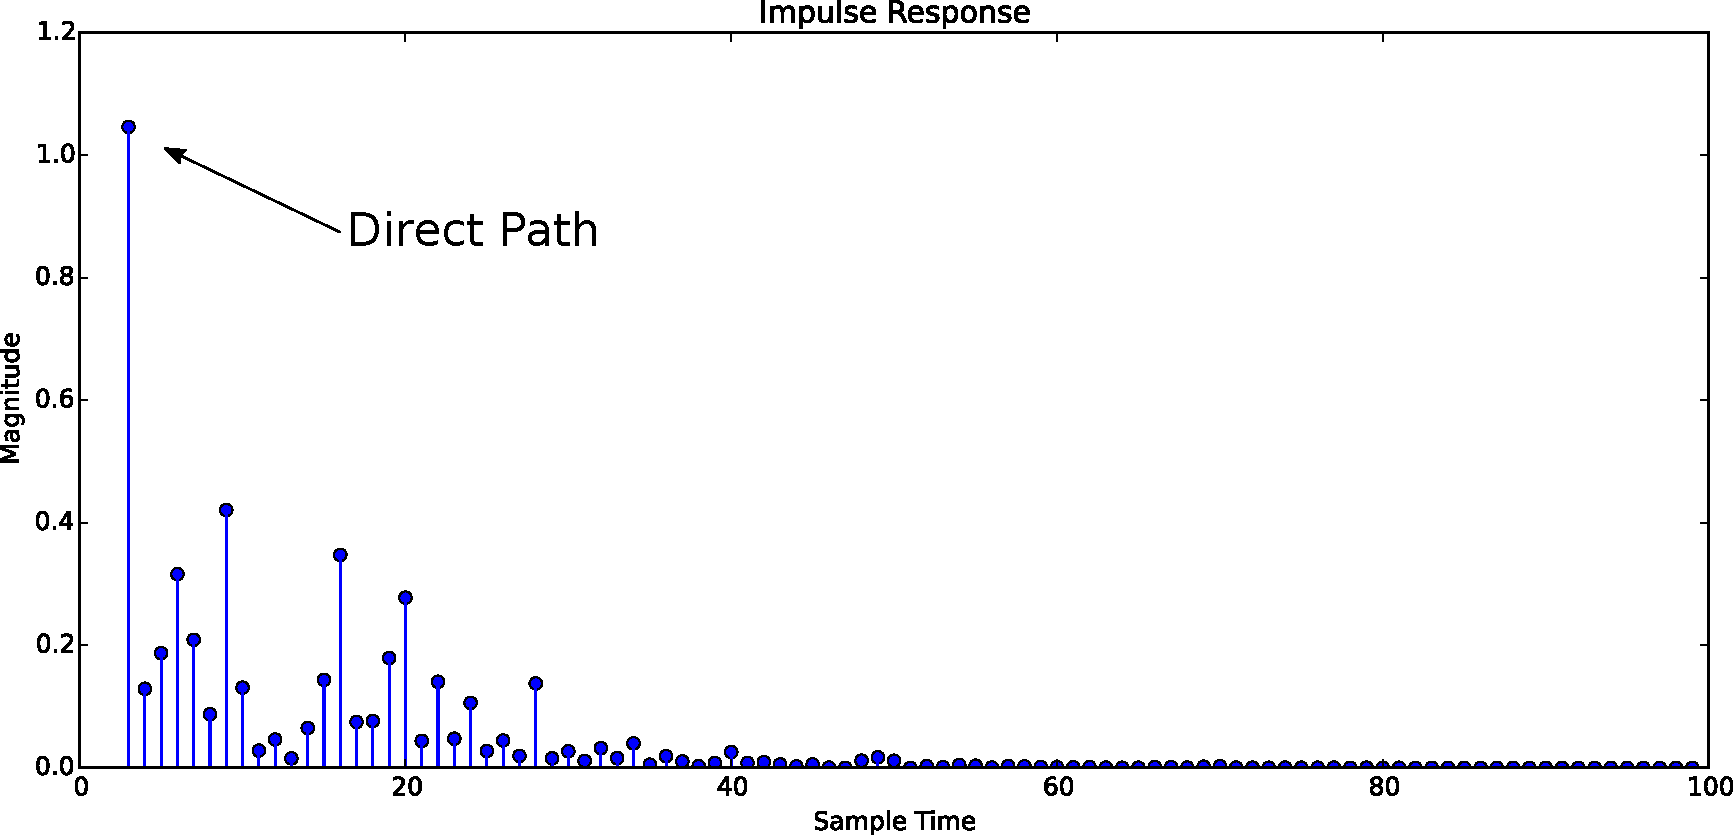
\includegraphics[width=\textwidth]{ImpulseResponse.pdf}
\end{figure}

\end{frame}


\begin{frame}{Convolution}

\begin{itemize}[label=$\vartriangleright$]
\item Add overlapping signals, {\em delayed} and {\em decayed}
\end{itemize}

\begin{figure}[t]
	\centering
    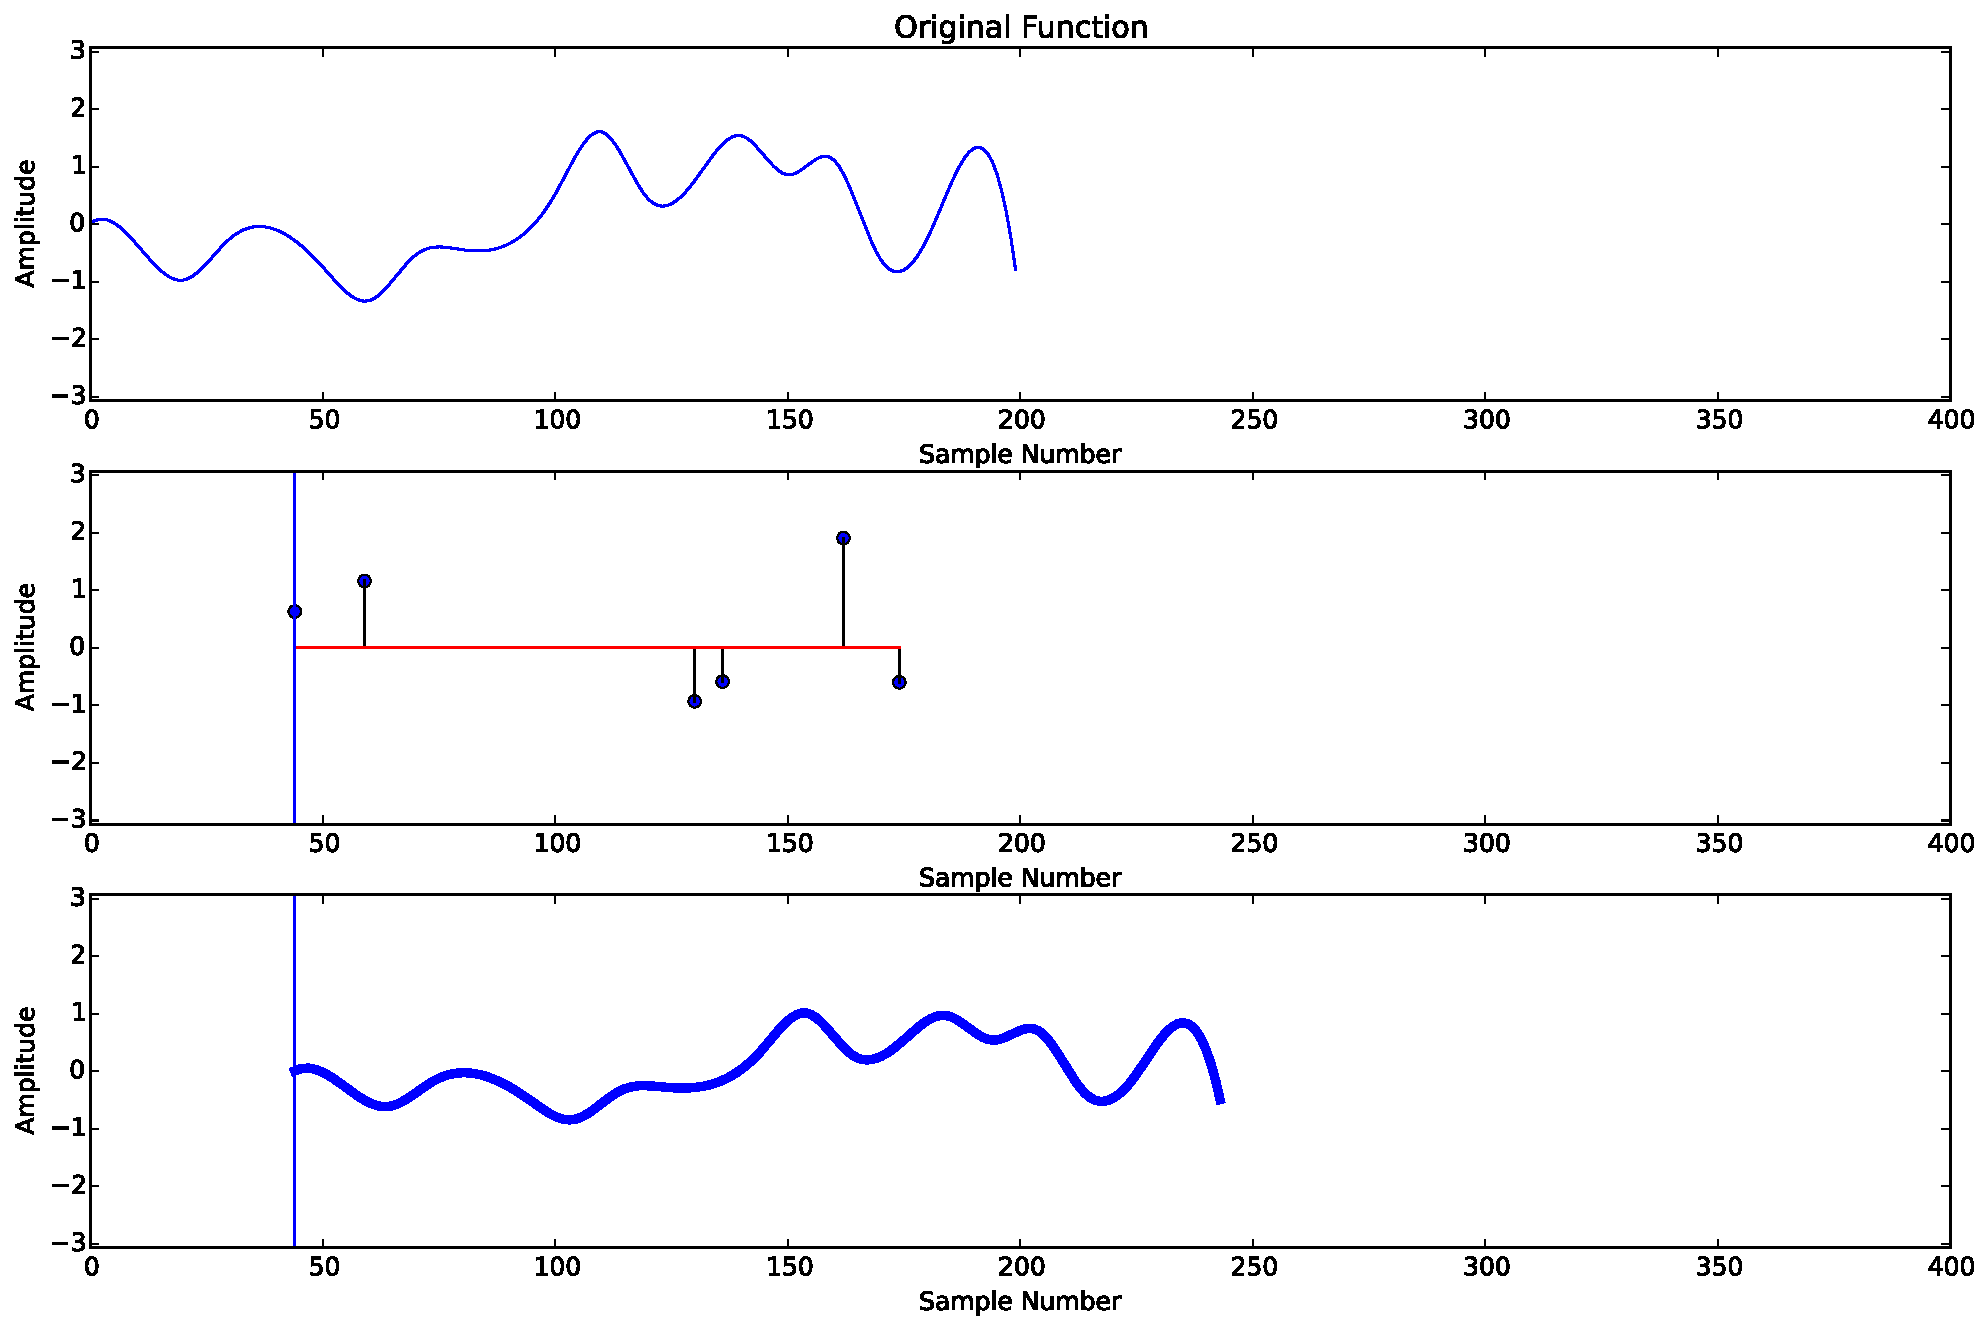
\includegraphics[width=\textwidth]{Conv0.pdf}
\end{figure}


\end{frame}


\begin{frame}{Convolution}

\begin{itemize}[label=$\vartriangleright$]
\item Add overlapping signals, {\em delayed} and {\em decayed}
\end{itemize}

\begin{figure}[t]
	\centering
    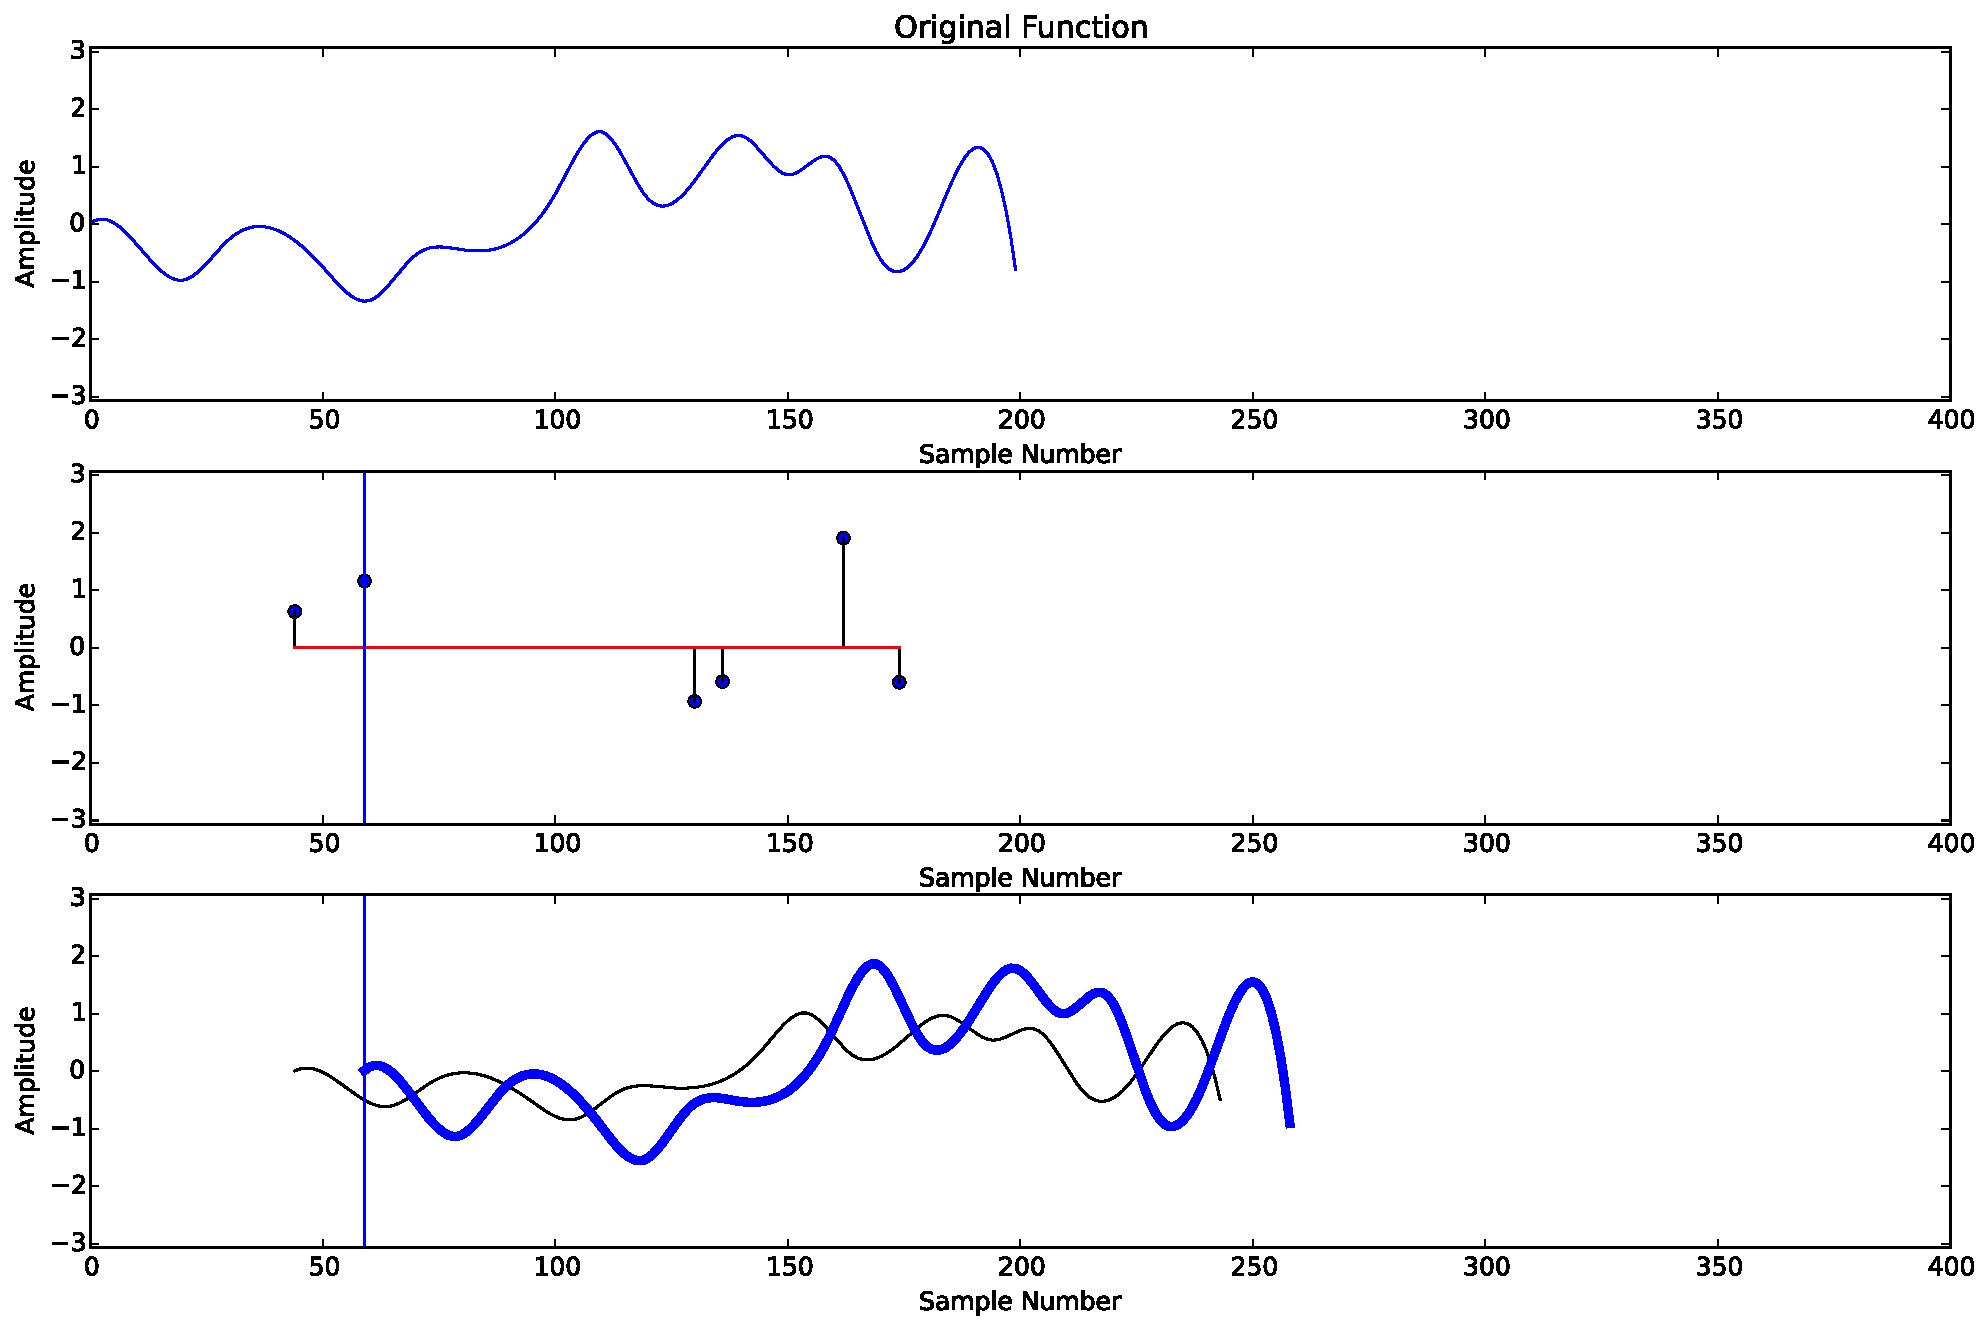
\includegraphics[width=\textwidth]{Conv1.pdf}
\end{figure}


\end{frame}


\begin{frame}{Convolution}

\begin{itemize}[label=$\vartriangleright$]
\item Add overlapping signals, {\em delayed} and {\em decayed}
\end{itemize}

\begin{figure}[t]
	\centering
    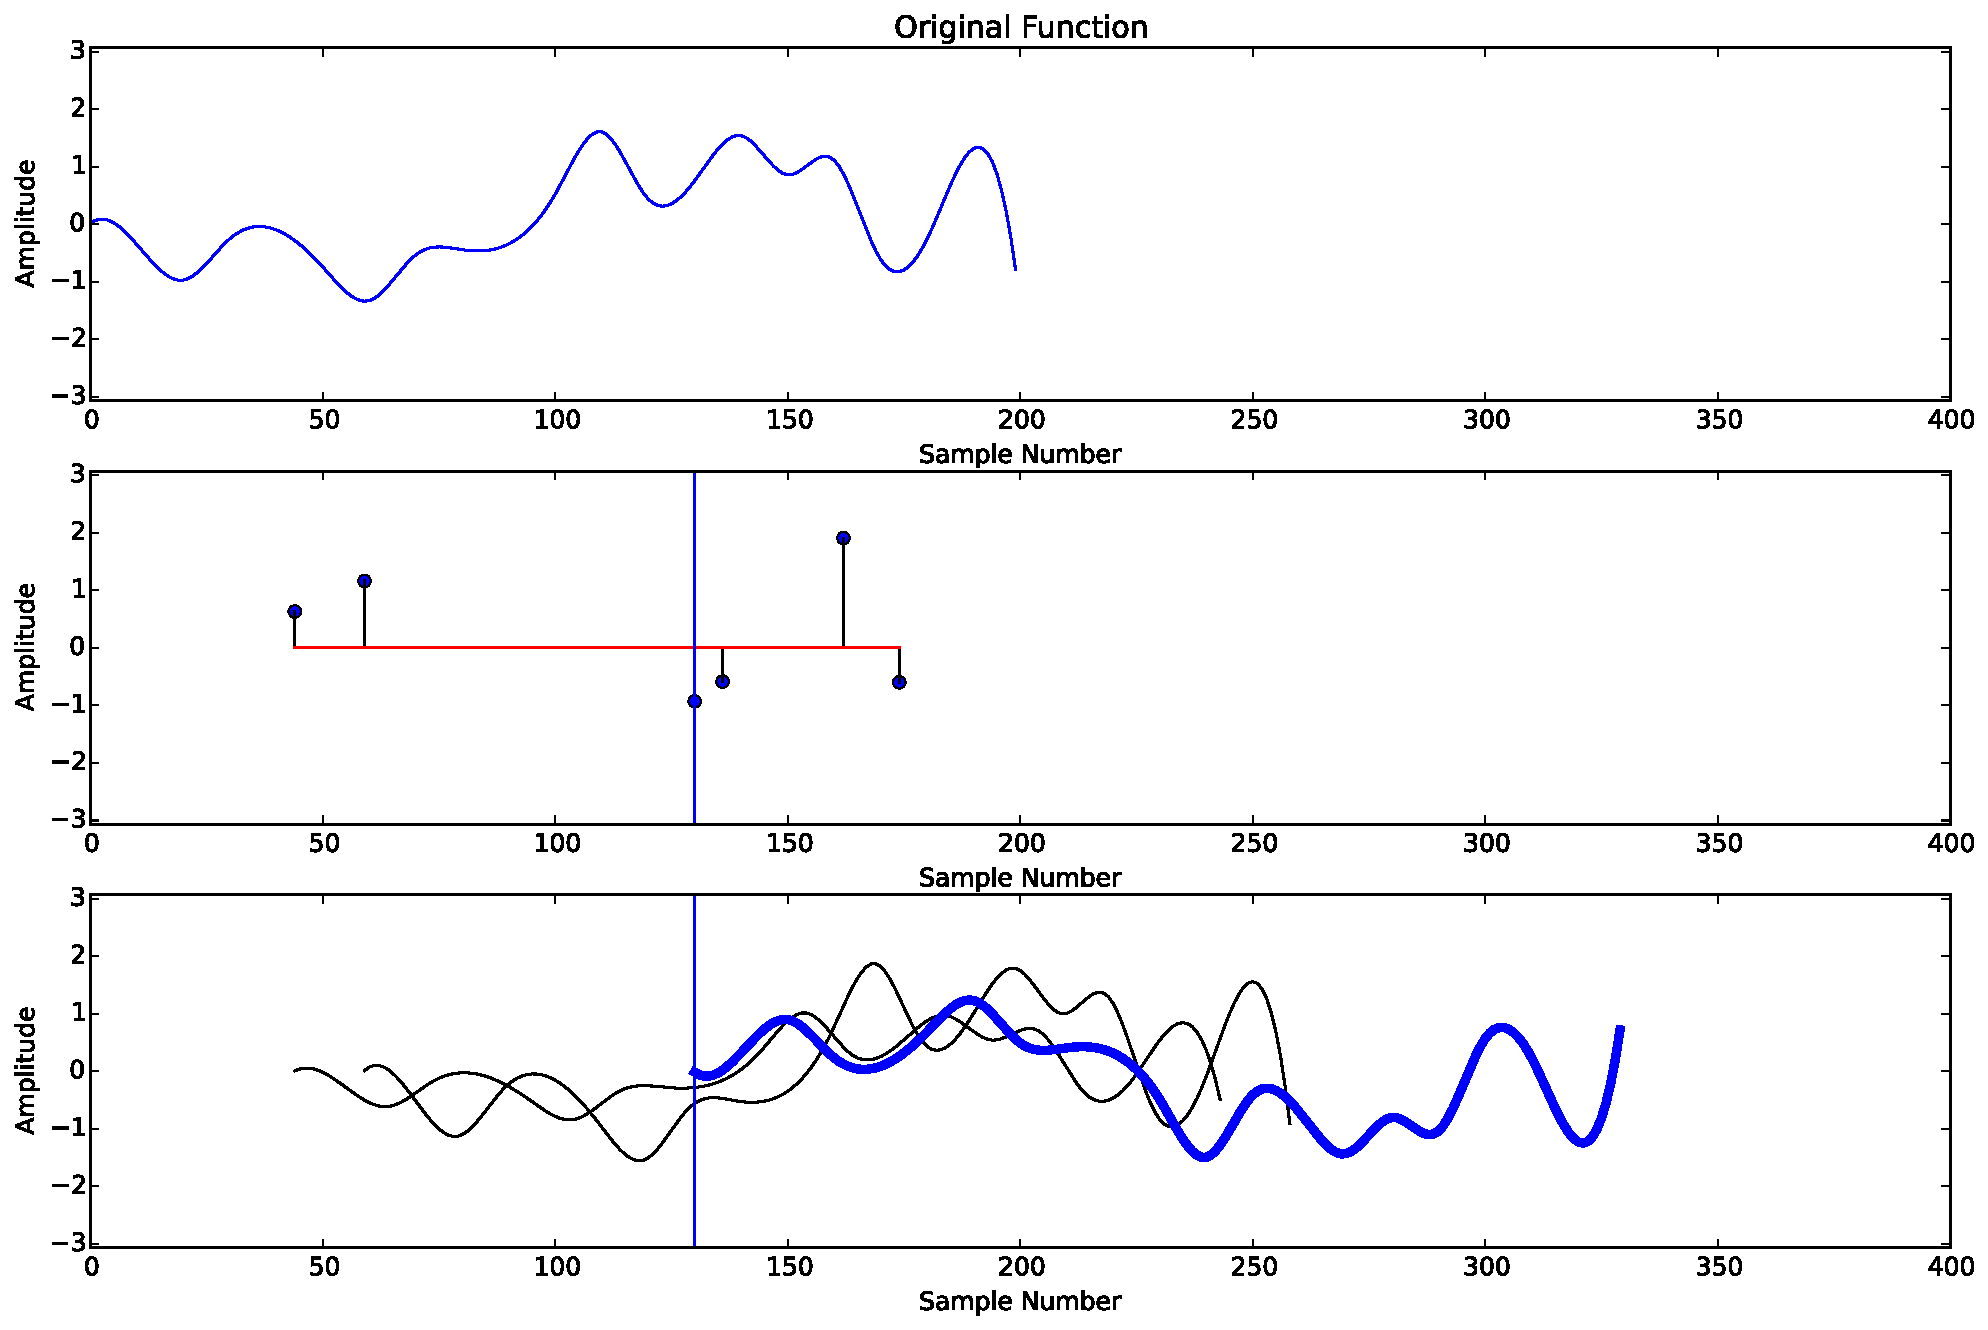
\includegraphics[width=\textwidth]{Conv2.pdf}
\end{figure}


\end{frame}



\begin{frame}{Convolution}

\begin{itemize}[label=$\vartriangleright$]
\item Add overlapping signals, {\em delayed} and {\em decayed}
\end{itemize}

\begin{figure}[t]
	\centering
    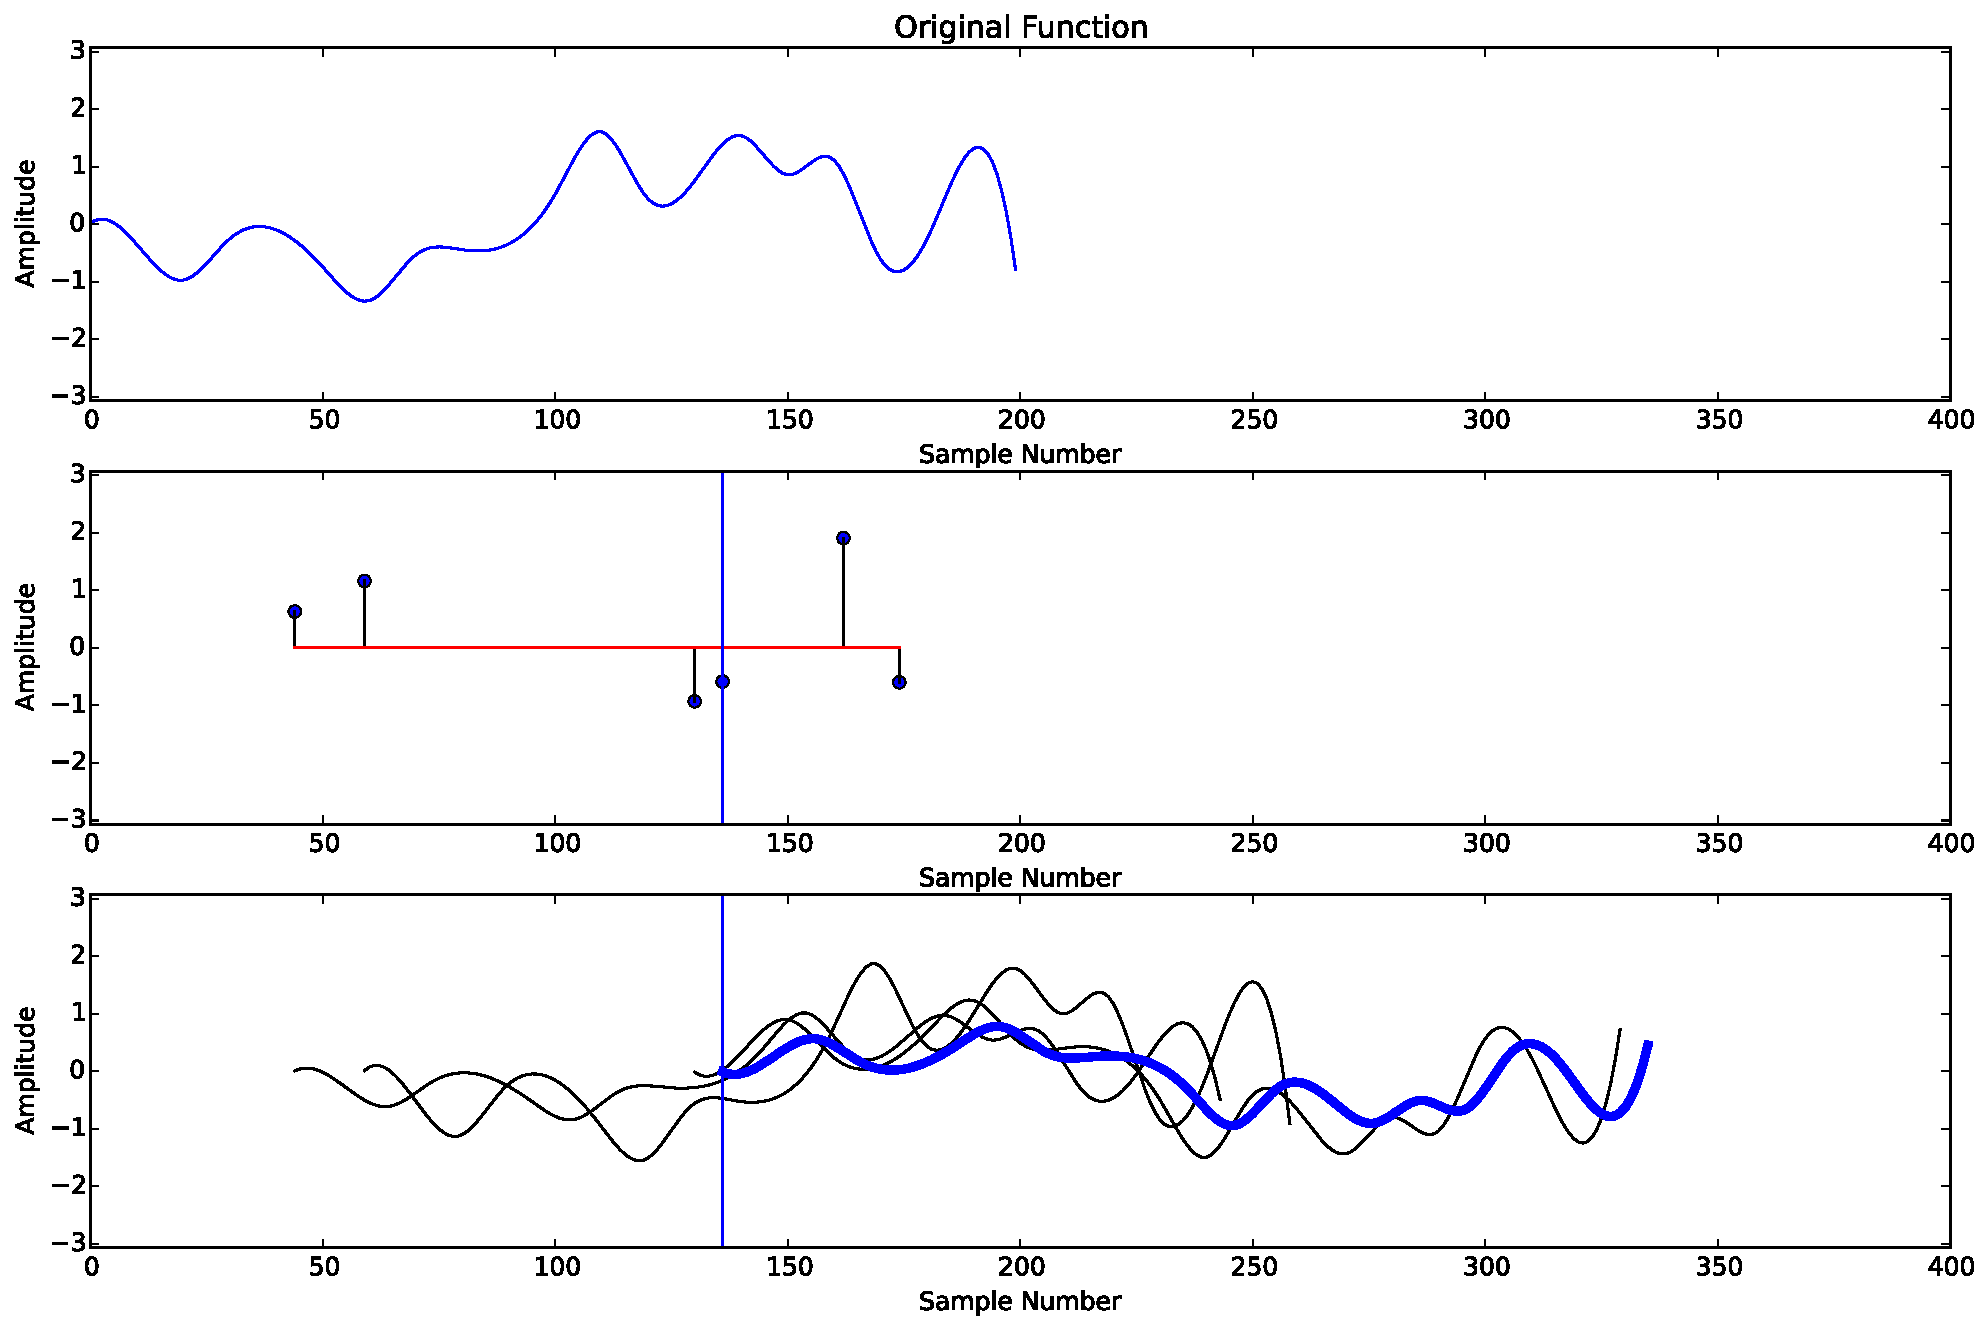
\includegraphics[width=\textwidth]{Conv3.pdf}
\end{figure}


\end{frame}


\begin{frame}{Convolution}

\begin{itemize}[label=$\vartriangleright$]
\item Add overlapping signals, {\em delayed} and {\em decayed}
\end{itemize}

\begin{figure}[t]
	\centering
    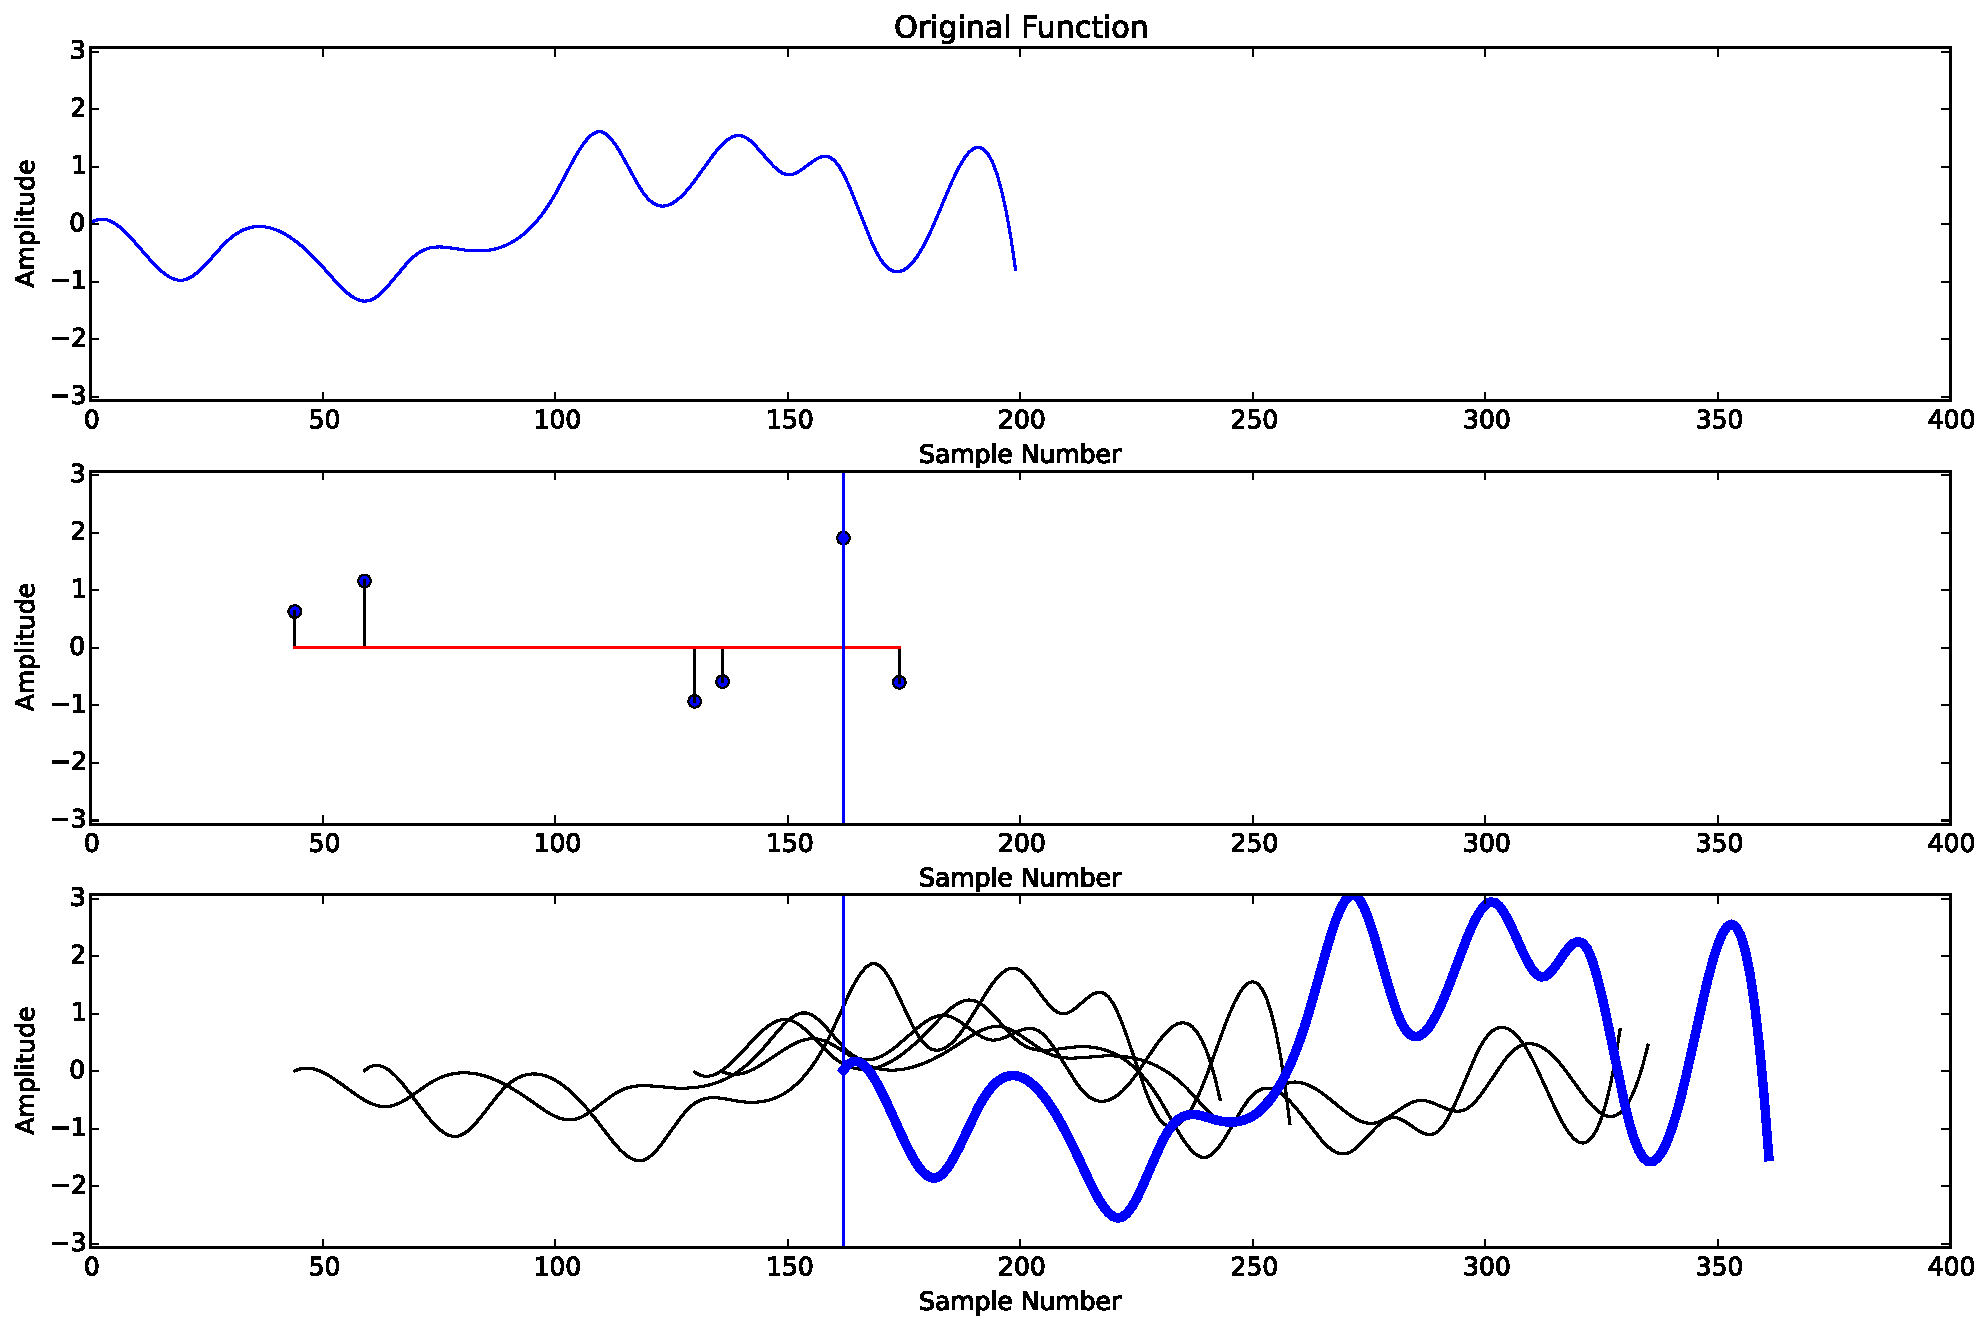
\includegraphics[width=\textwidth]{Conv4.pdf}
\end{figure}


\end{frame}

\begin{frame}{Convolution}

\begin{itemize}[label=$\vartriangleright$]
\item Add overlapping signals, {\em delayed} and {\em decayed}
\end{itemize}

\begin{figure}[t]
	\centering
    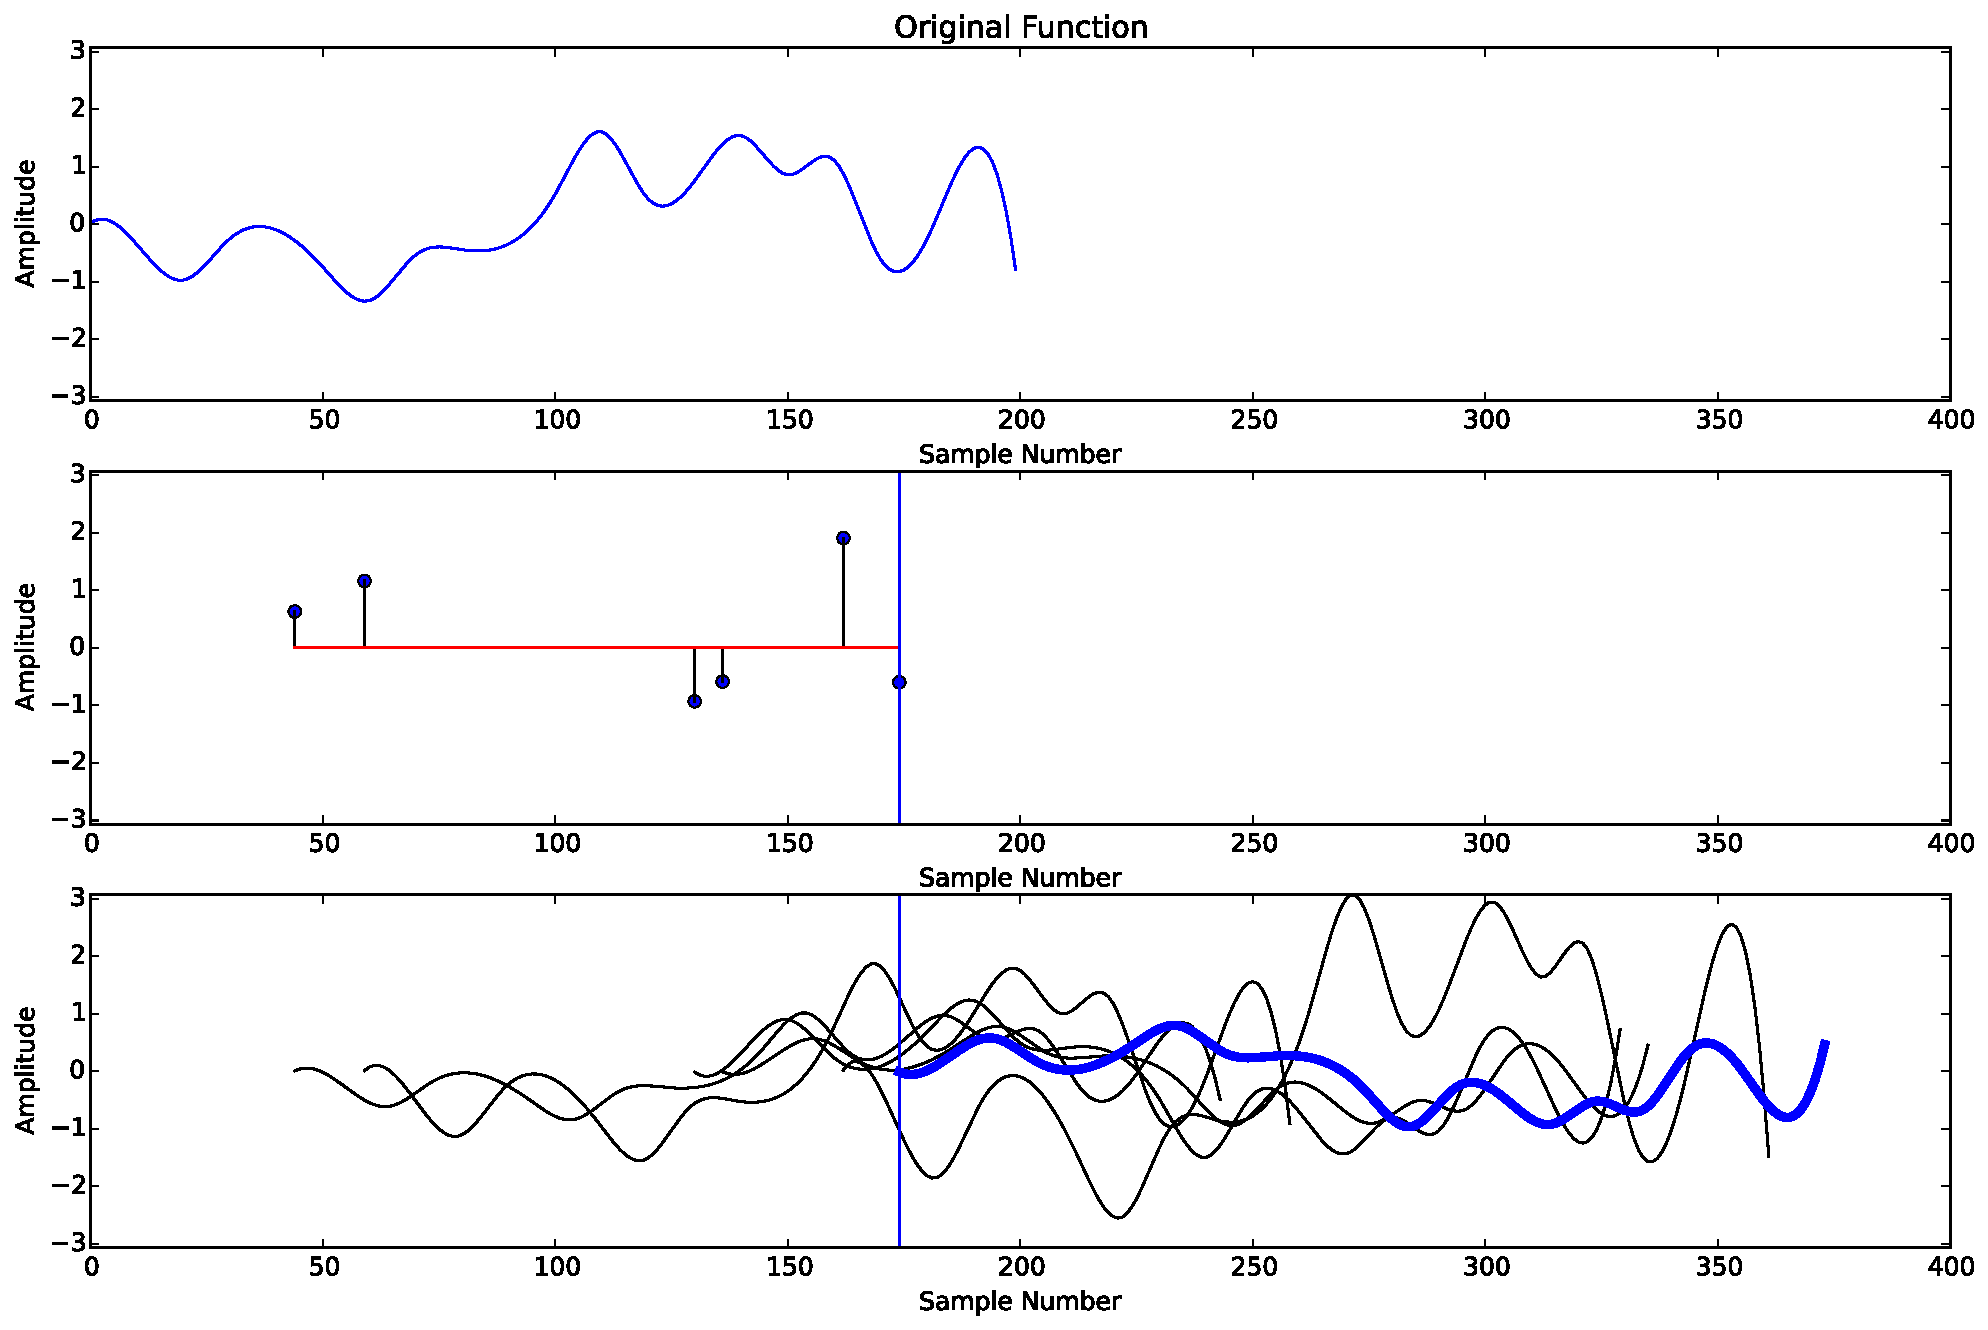
\includegraphics[width=\textwidth]{Conv5.pdf}
\end{figure}


\end{frame}

\begin{frame}{Convolution: Result}

\begin{itemize}[label=$\vartriangleright$]
\item Add overlapping signals, {\em delayed} and {\em decayed}
\end{itemize}

\begin{figure}[t]
	\centering
    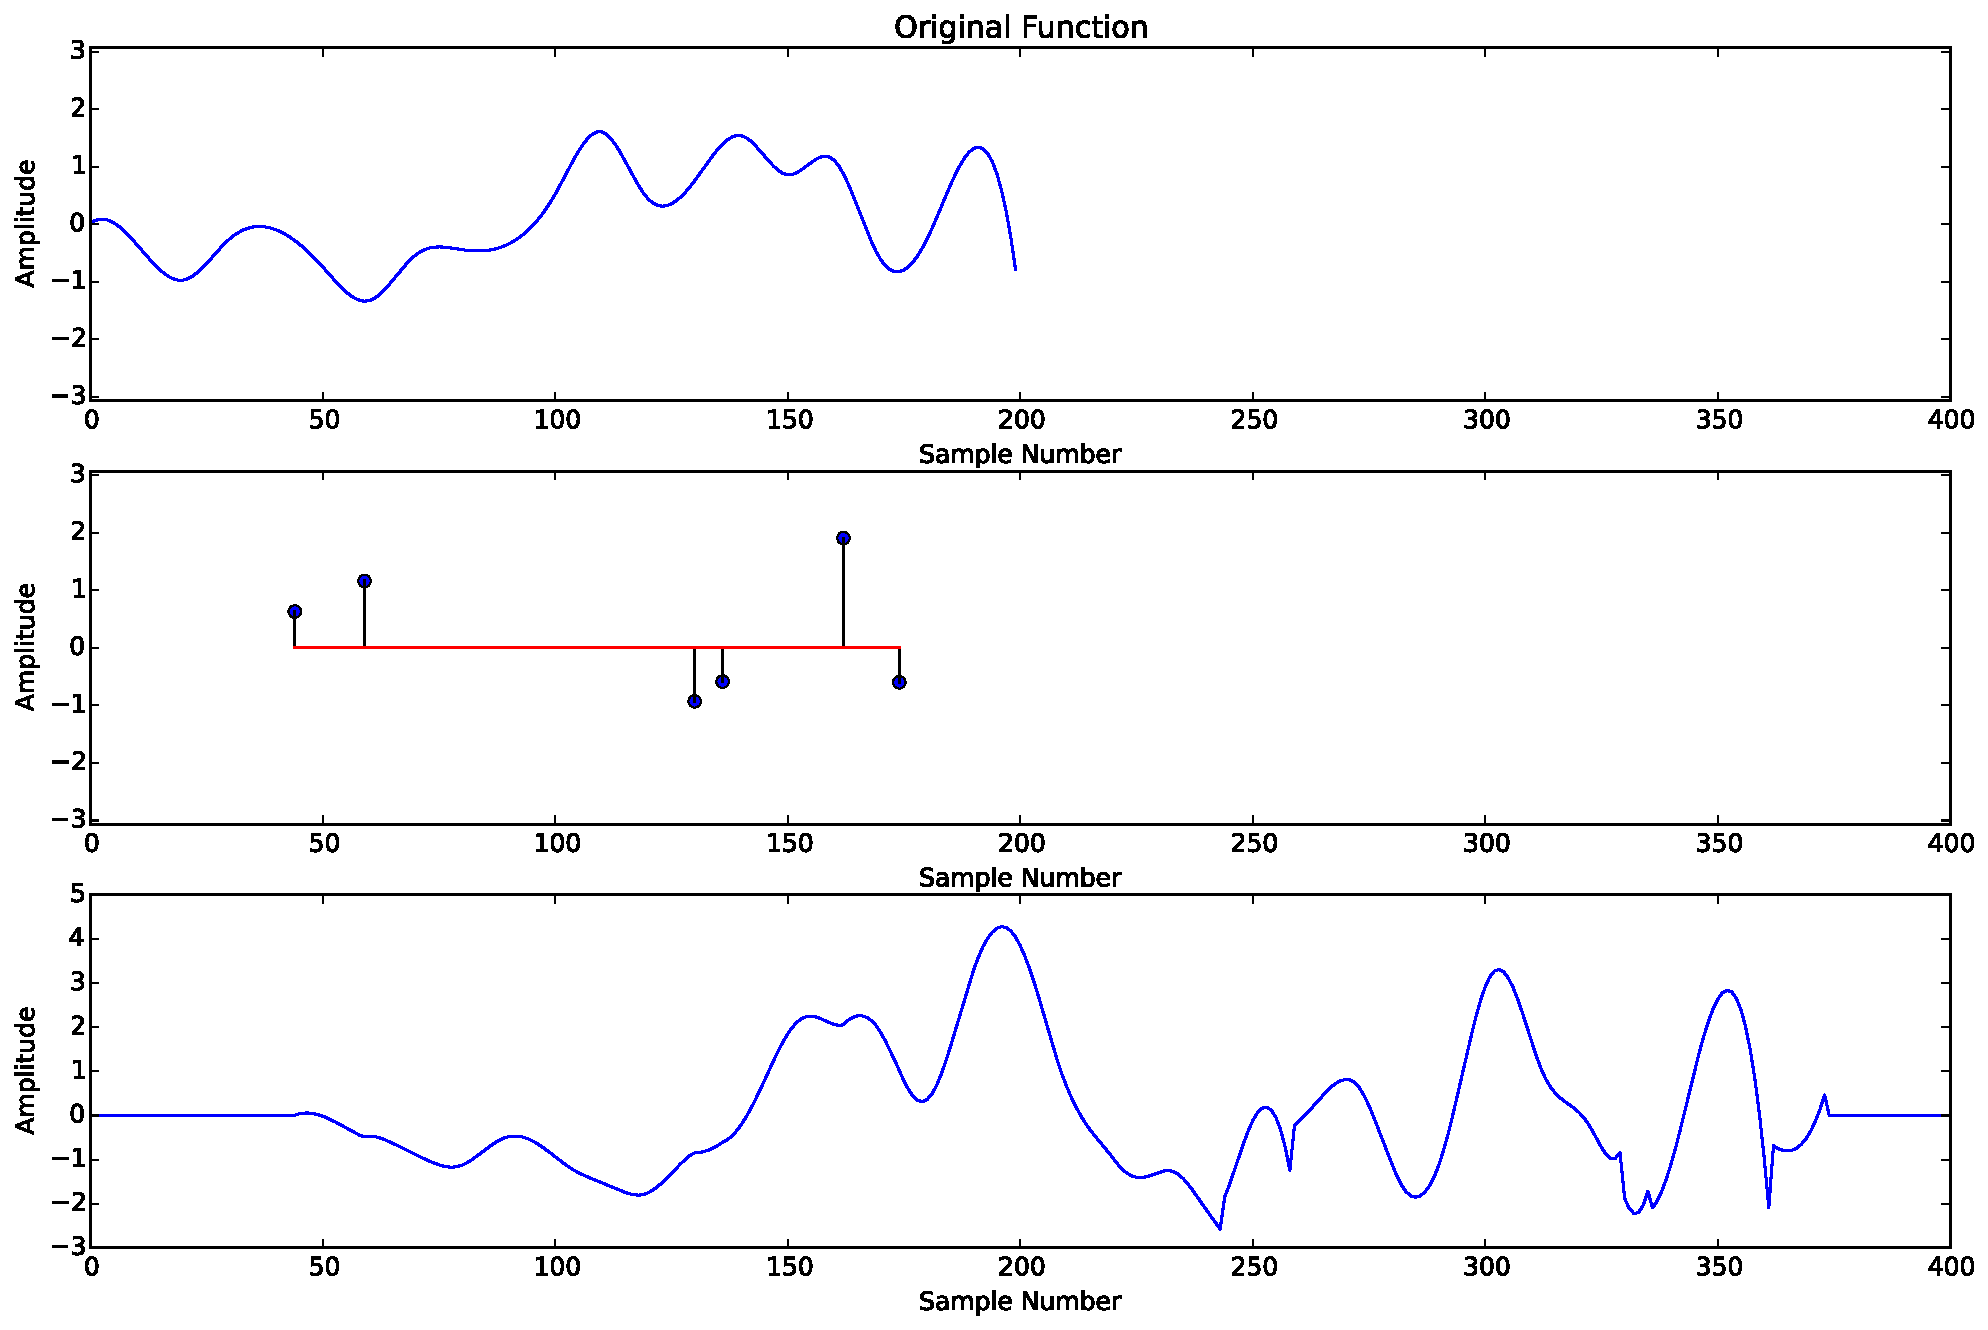
\includegraphics[width=\textwidth]{ConvResult.pdf}
\end{figure}


\end{frame}


\begin{frame}{Convolution: Notation / Equation}

$x[n]$: Discretely sampled signal describing the sound

$h[n]$: Discretely sampled signal describing impulse

\begin{figure}[t]
	\centering
    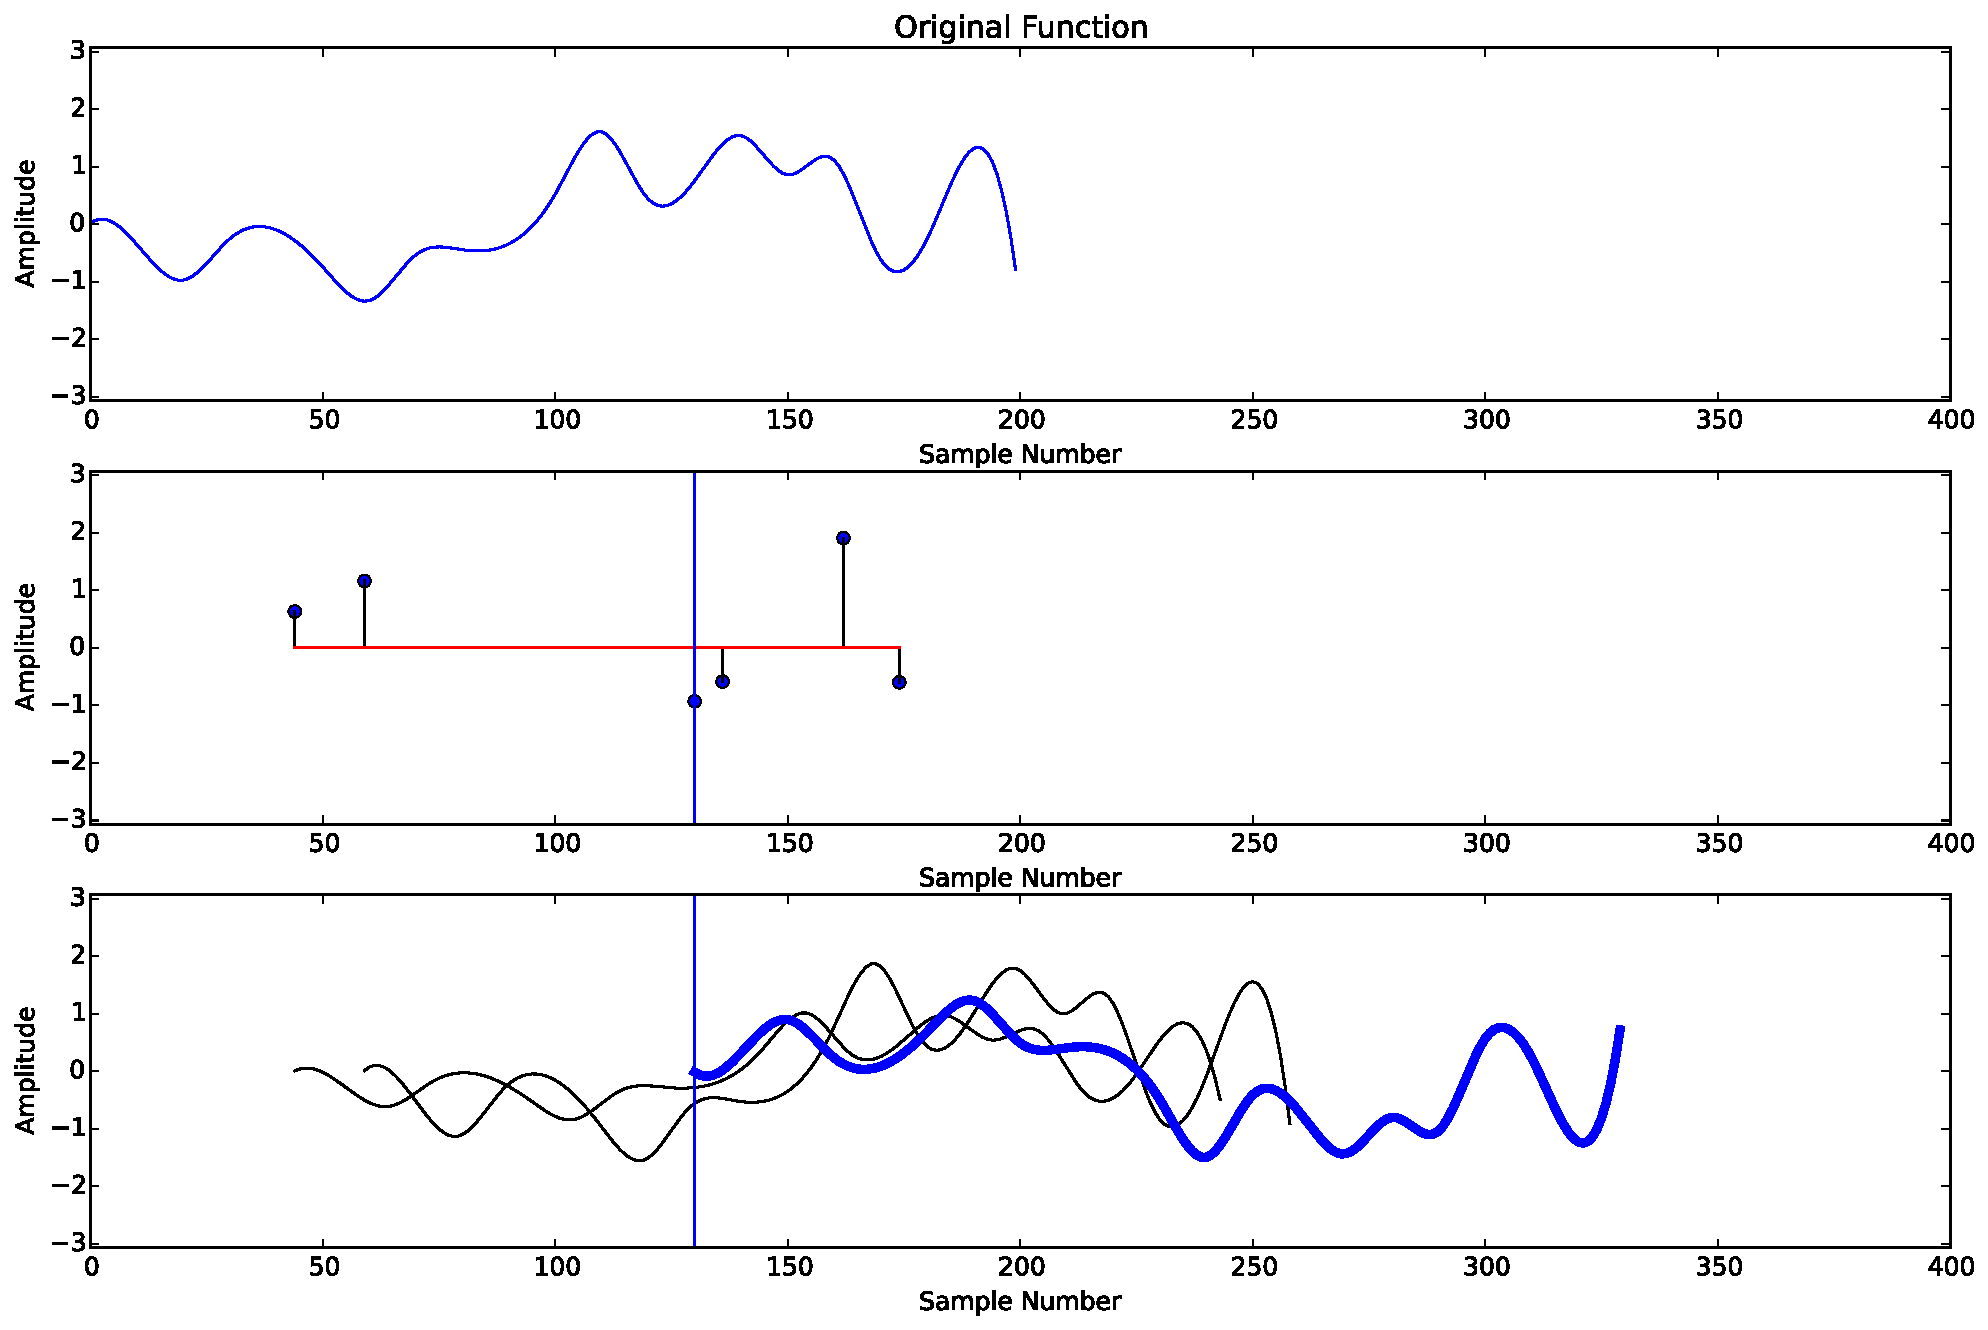
\includegraphics[width=0.8\textwidth]{Conv2.pdf}
\end{figure}

\end{frame}

\begin{frame}{Convolution: Notation / Equation (RAFFLE POINT)}

$x[n]$: Discretely sampled signal describing the sound

$h[n]$: Discretely sampled signal describing impulse

\begin{figure}[t]
	\centering
    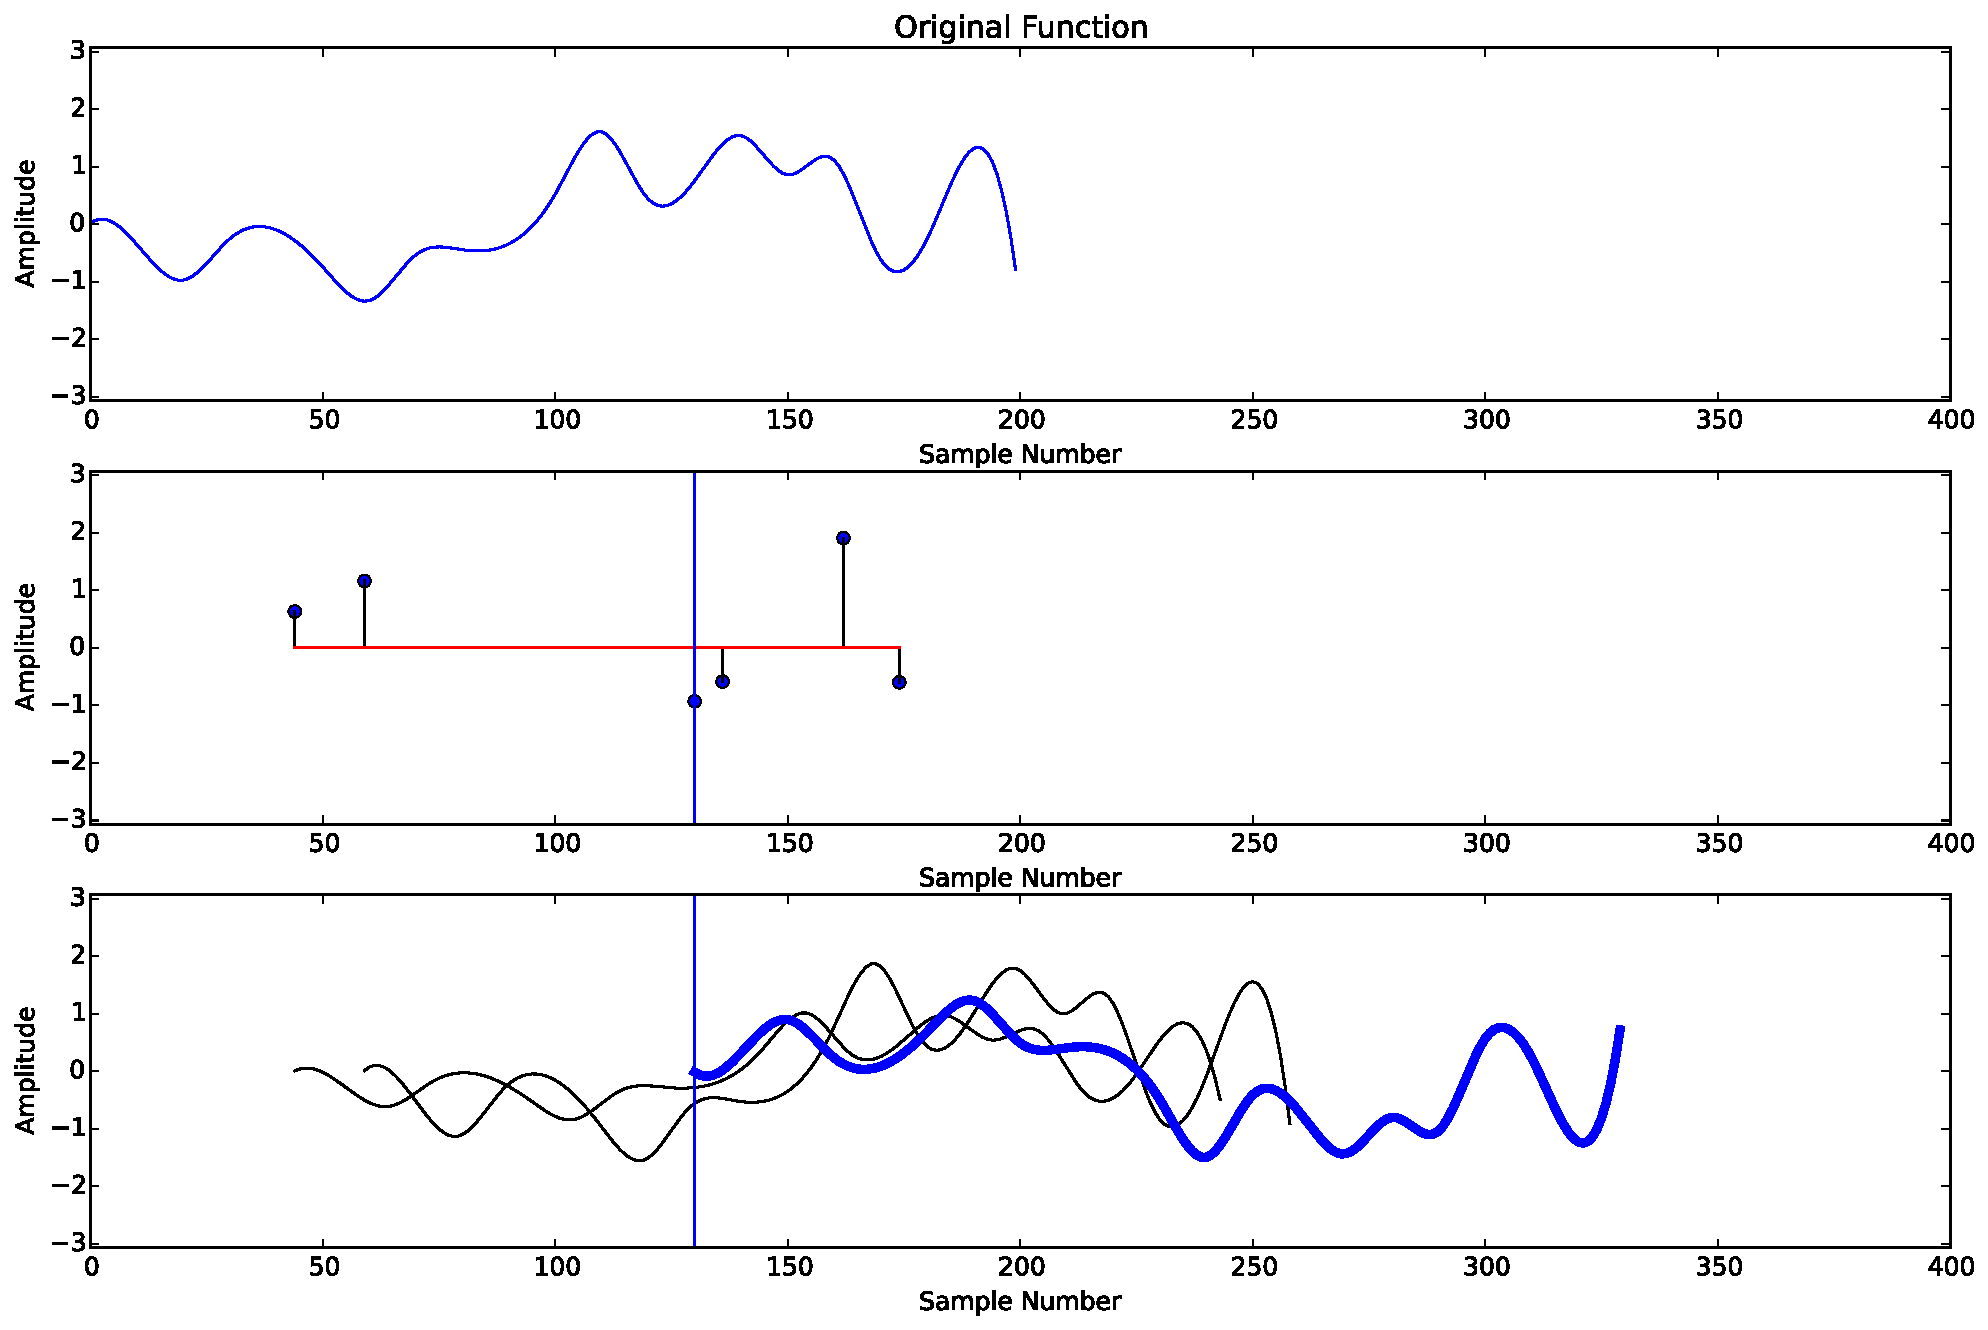
\includegraphics[width=0.8\textwidth]{Conv2.pdf}
\end{figure}

\end{frame}

\begin{frame}{Convolution: Notation/Equation}

$x[n]$: Discretely sampled signal describing the sound

$h[n]$: Discretely sampled signal describing impulse

\[ (x*h)[n] = \sum_{k=0}^N h[k]x[n-k] \]

\uncover<2->{
Roles can switch!
}

\end{frame}

\begin{frame}{Gaussian Interpolation}

Given non-integer bin index $n_0$ with amplitude $a$

\[ h[n] = a e^{-(n-n_0)^2/2\sigma^2} / \left(\sum_{k = -2\sigma}^{k=2\sigma} e^{-(n-n_0)^2/2\sigma^2} \right) \]

\begin{figure}[t]
	\centering
    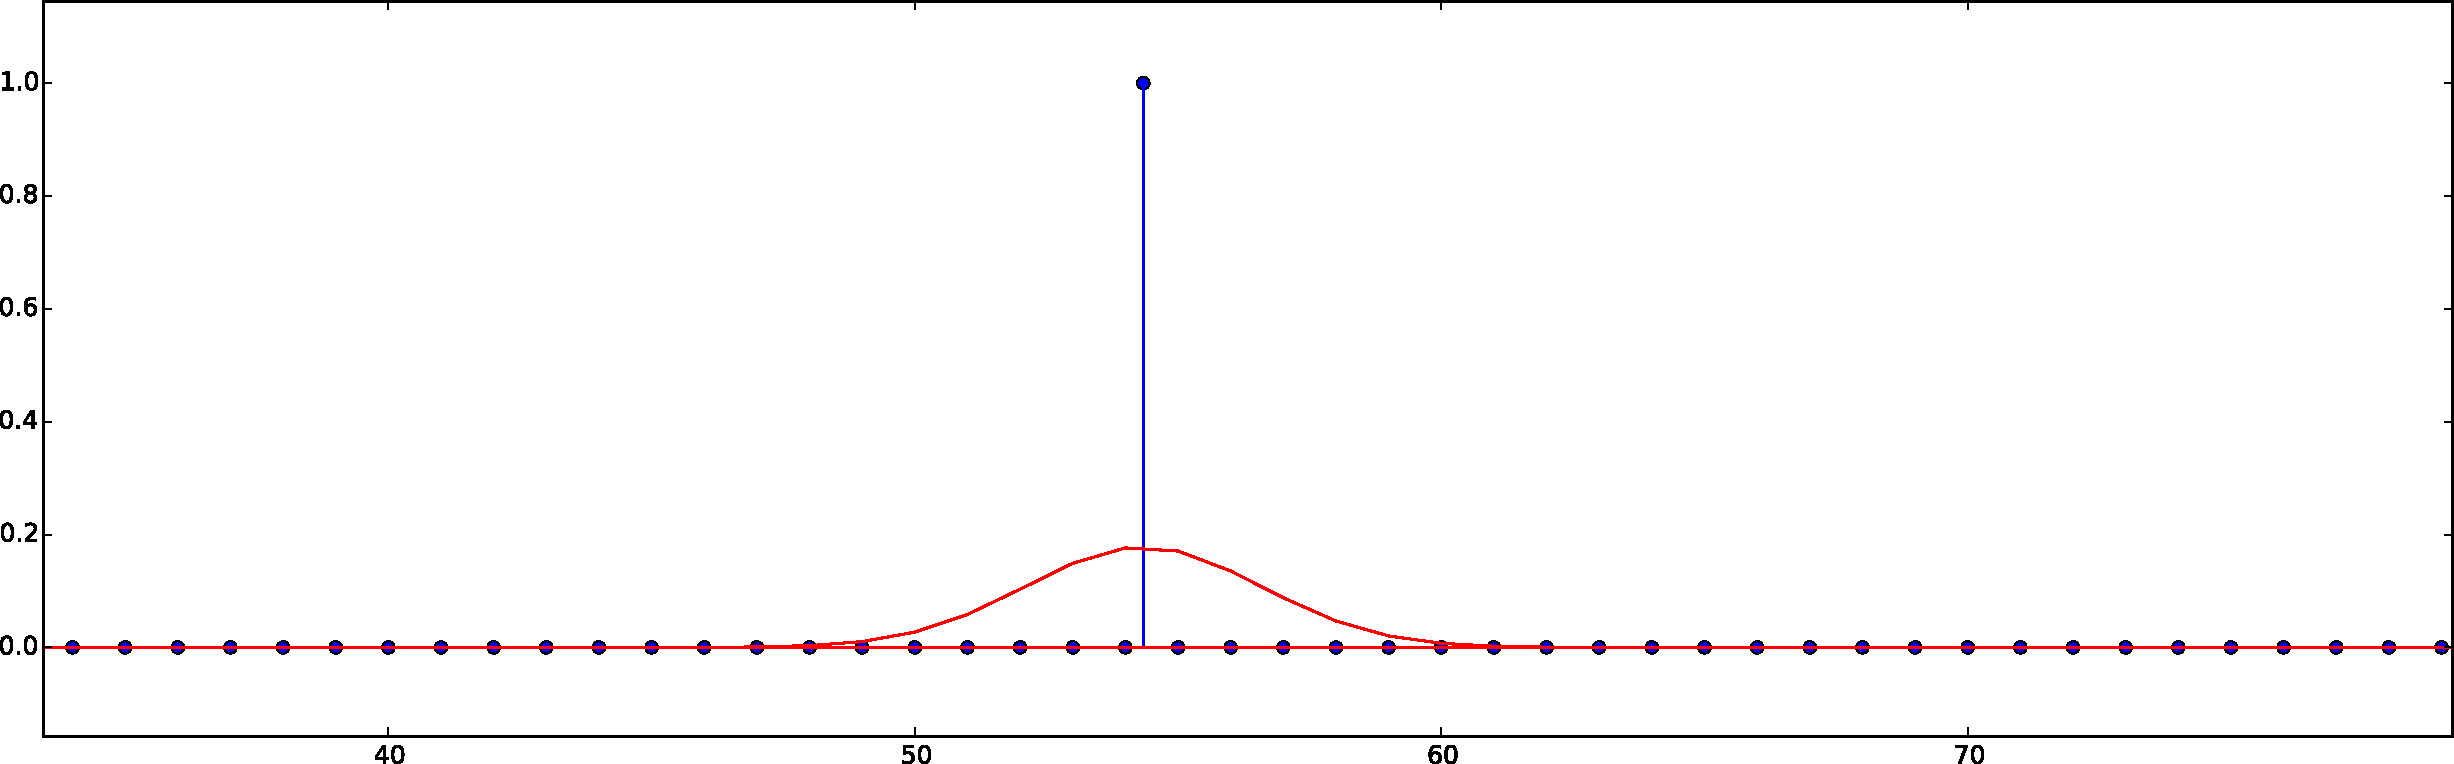
\includegraphics[width=0.8\textwidth]{GaussInterp.pdf}
\end{figure}


\end{frame}

\begin{frame}{Convolution Examples}

Interactive demo

\end{frame}


\begin{frame}{Table of Contents}

\begin{itemize}[label=$\vartriangleright$]
	\item 3D Rotations Continued
    \item Image Sources
	\item Convolution
\end{itemize}
\begin{itemize}[label=$\blacktriangleright$]
	\item Scene Graphs
\end{itemize}


\end{frame}


\begin{frame}{Scene Graph: Human body}

\begin{figure}[t]
	\centering
    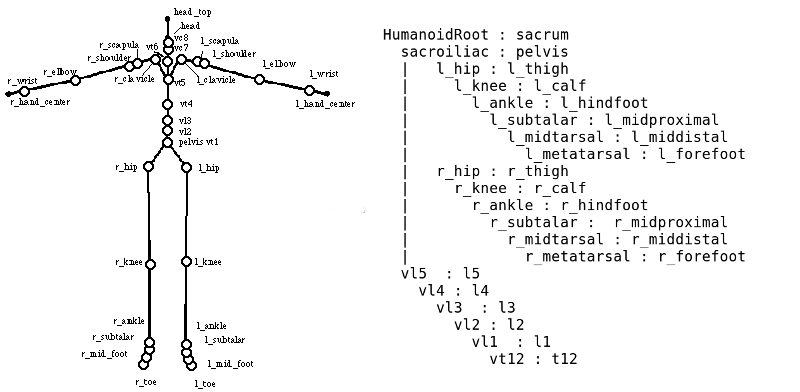
\includegraphics[width=\textwidth]{MPEG4Diagram.png}
\end{figure}


\tiny Figure courtesy of \url{http://www.euclideanspace.com/physics/kinematics/joints/}

\end{frame}

\begin{frame}{Scene Graph: Human body}

MOCAP interactive example

\end{frame}

\begin{frame}{Scene Graph: Bedroom}

\begin{figure}[t]
	\centering
    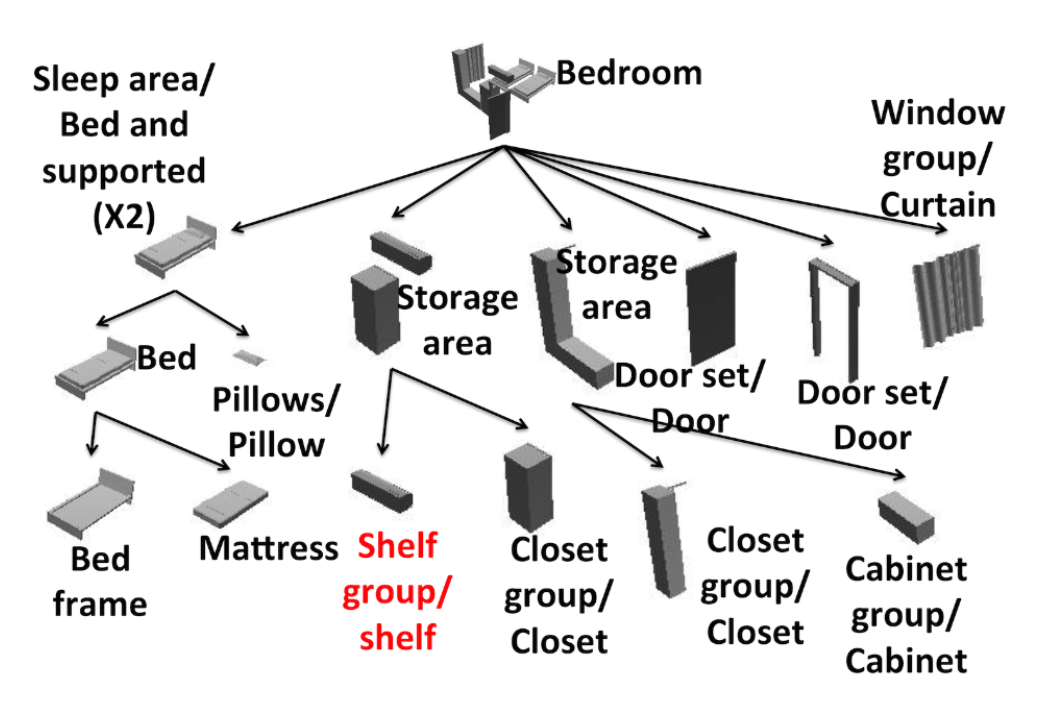
\includegraphics[width=0.8\textwidth]{SceneGraphBedroom.png}
\end{figure}

\tiny Liu, Tianqiang, et al. "Creating consistent scene graphs using a probabilistic grammar." ACM Transactions on Graphics (TOG) 33.6 (2014): 211.

\end{frame}

\begin{frame}{Scene Graph: Library}

\begin{figure}[t]
	\centering
    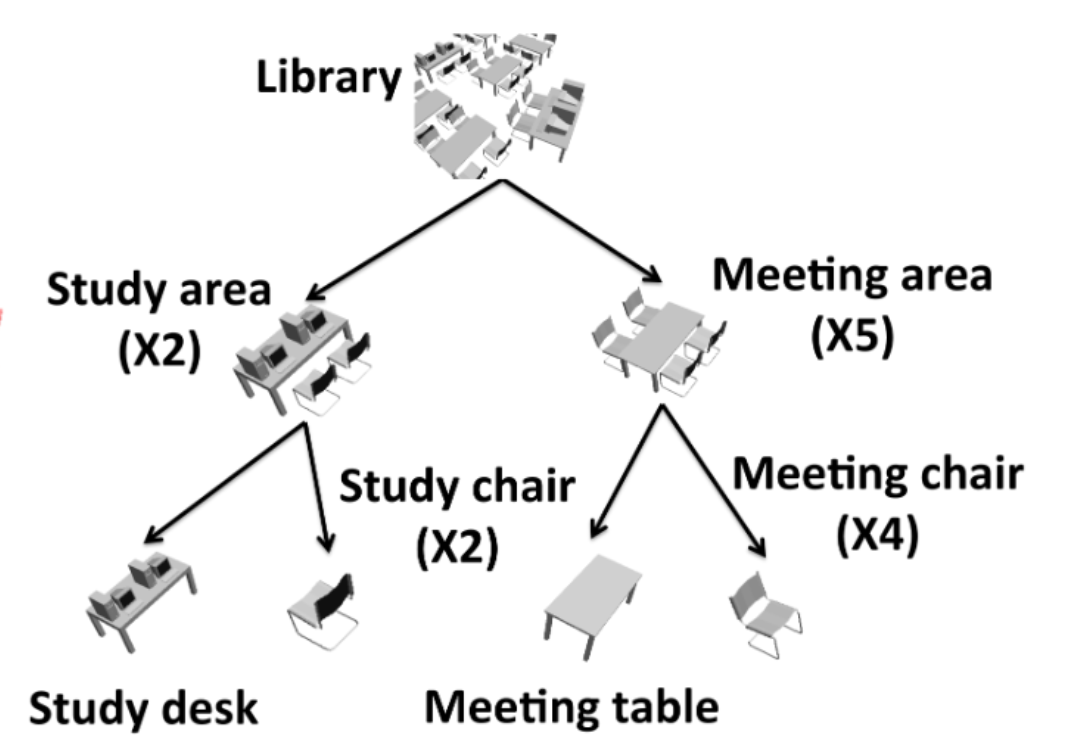
\includegraphics[width=0.8\textwidth]{SceneGraphLibrary.png}
\end{figure}

\tiny Liu, Tianqiang, et al. "Creating consistent scene graphs using a probabilistic grammar." ACM Transactions on Graphics (TOG) 33.6 (2014): 211.

\end{frame}

\begin{frame}{Scene Graph: Euler Angles Visualization}

\end{frame}

\begin{frame}{Designing Scene Graphs}

Interactive Example

\end{frame}

%\begin{figure}[t]
%    \captionsetup[subfloat]{labelformat=empty}
%	\centering
%	\subfloat[Before]{
%	    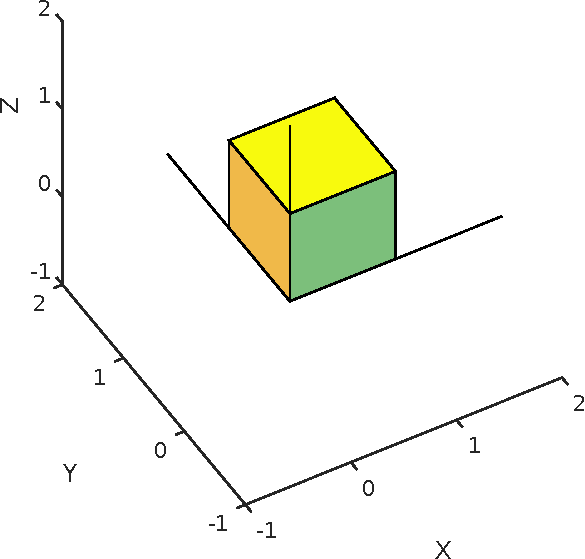
\includegraphics[width=0.46\textwidth]{CubeOrig.pdf}
%	}
%	\subfloat[After]{
%	    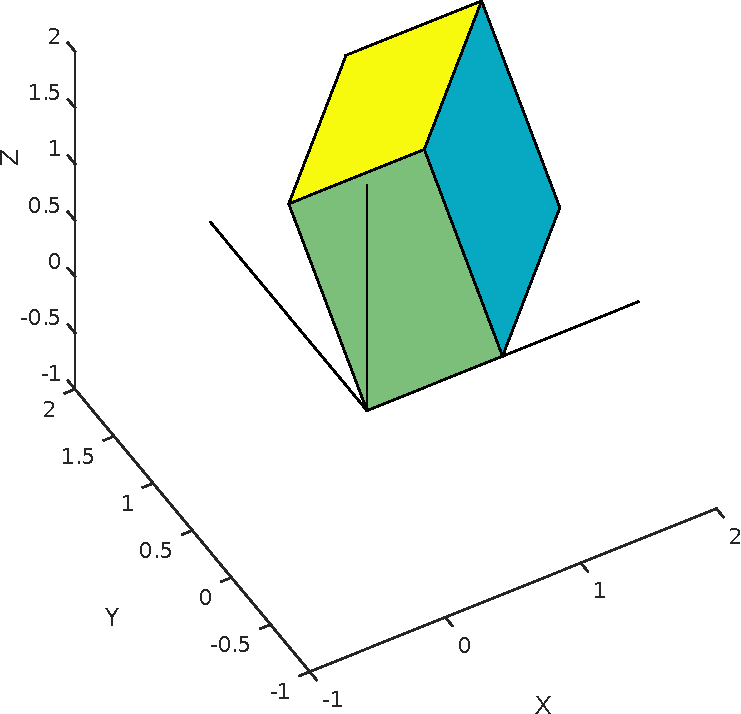
\includegraphics[width=0.46\textwidth]{ShearXY.pdf}
%	}

%\end{figure}


\end{document}

